%%%%%%%%%%%%%%%%%%%%%%%%%%%%%%%%%%%%%%%%%%%%%%%%%%%%%%%%%%%%%%%%%
%%%%%%%%%%%%%%%%%%%%%%%%%%%%%%%%%%%%%%%%%%%%%%%%%%%%%%%%%%%%%%%%%
%%%%%%%%%%%%%%%%%%%%%%%%%%%%%%%%%%%%%%%%%%%%%%%%%%%%%%%%%%%%%%%%%

\chapter{Short Introduction to Programming in Java}
\label{chap:IntroJava}

%%%%%%%%%%%%%%%%%%%%%%%%%%%%%%%%%%%%%%%%%%%%%%%%%%%%%%%%%%%%%%%%%
\section{Programming in Java}
\label{sec:Programming}


\subsection{General Considerations}
\label{sec:General_considerations}
This book is about stochastic simulation methods and their applications to
physical systems. The material is presented at an introductory level. We do 
not assume any prior knowledge on probability theory or on the theory of 
stochastic processes. We assume only the material known from the introductory 
courses in theoretical physics. The style of the presentation will be as 
informal as possible and as precise as necessary.



\subsection{Programming Languages -- Why Java ?}
\label{sec:Programming_languages}
It is clear that it is not possible to teach simulation methods without 
performing some numerical experiments in the classroom and that it is 
impossible for the students to learn stochastic simulation methods without 
implementing the algorithms. Therefore, the theory and the corresponding 
algorithms will be presented in a highly interconnected, and, we 
hope, organic way.

In order to stick to this idea it was necessary to choose a programming 
language. The obvious criteria for taking such a decision are
\cite[]{GARCIA}
\begin{enumerate}
\item Efficiency,
\item Understandability,
\item Good graphics,
\item Standard/Portable,
\item Cost,
\item Parallelizability.
\end{enumerate}
The first criterion is of course very important because already simple 
stochastic algorithms require a considerable amount of CPU time.
A secondary aim of the course is to make the student acquainted with a 
programming language ``in action'' so they should learn something 
about a ``good 
programming style'' for real-life problems. Visualization of the results 
obtained allows to understand in a plastic way what is going on physically. So 
the interface between program and visualization tool/graphical output should
be comfortable. Last not least the availability of the program should be
guaranteed. The corresponding compilers should be available at low, in the 
ideal case at no cost to the students for home exercises. Furthermore, they
should be portable on PCs with Windows or Linux operating systems, on Macintosh
and on workstations from the UNIX world (IBM AIX, Solaris, SGI Irix, ...).
Since almost all universities do have a high--performance parallel computer 
the language should also allow to demonstrate high--performance parallel 
algorithms.

Because of our background of convinced Fortran users we considered the 
following alternatives: our beloved Fortran, MATLAB, a language which 
is popular in 
the engineering and applied mathematics communities, and Java, the 
"Wunderkind" of software developers and of the Internet community. We have 
not considered C, C++ for the simple reason that we never felt the necessity 
to learn them.

All the languages considered  in some sense satisfy the above criteria. All
are more  or less portable on different platforms (at different expenses), all
allow the use of good visualization tools (at different prices), and, of 
course, all are clean. But not all are equally powerful. 

We checked the power (the efficiency) of the languages considered by the 
following benchmark, which represent the prototype of a stochastic simulation. 
We generated 100 trajectories of a typical one-step stochastic process
and compared the CPU times obtained by different languages. The result
of the benchmarks are summarized in the following table. The listings
of the corresponding programs are listed in the appendix.

\begin{table}[htbp]
  \begin{center}
    \leavevmode
    \begin{tabular}{llp{3cm}|c|c}
      Language & OS & Software & Machine & CPU time \\\hline\hline  
   Fortran 90 & Linux & Nag f90 Compiler V2.2(260) & Pentium 133 & 2.1 sec.\\
           & Linux & Nag f90 Compiler V2.2(260) with -O3 & Pentium 133 & 2.4 sec.\\
           & Linux & Nag f95 Compiler V1.0(436) & Pentium 133 & 2.3 sec.\\
           & Linux & Nag f95 Compiler V1.0(436) wiht -O4& Pentium 133 & 2.3 sec.\\
           & Linux & Pallas f95 Compiler V3.0-3 & Pentium 133 & 1.3 sec.\\
           & Linux & Pallas f95 Compiler V3.0-3 & Pentium 133 & 1.4 sec.\\\hline
   C       & Linux & GCC 2.7.2.3 & Pentium 133 & 2.1 sec. \\
           & Linux & GCC 2.7.2.3 with -O3 & Pentium 133 & 2.0 sec. \\\hline
   C++     & Linux & egcs-1.0.3 & Pentium 133 & 2.2 sec. \\
           & Linux & egcs-1.0.3 with -O3 & Pentium 133 & 1.8 sec. \\\hline
      Java & Linux & JDK 1.1.6v4 & Pentium II 333 & 6 sec. \\\hline
           & Linux & using JIT TYA (V1.0) & Pentium II 333 & 3 sec.\\
           & Linux &           & Pentium 133 & 16 sec. \\
           & Linux & using JIT TYA (V1.0) & Pentium 133 & 10 sec.\\
           & Linux &           & Pentium 200 MMX & 9 sec. \\
           & Linux & JDK 1.1.7 without JIT & DEC Alpha 21164 600 & 6 sec. \\
           & Win95 & JDK 1.1.7 using Symantec JIT & Pentium 133 & 9 sec. \\
           & Win95 & JDK 1.1.7 without JIT & Pentium 133 & 19 sec. \\
           & Win95 & JDK 1.2 using Symantec JIT & Pentium 133 & 8 sec. \\
           & Win95 & JDK 1.2 without JIT & Pentium 133 & 22 sec. \\\hline
   Matlab  & Win95 & Matlab 5.1 & Pentium 166 & 330 sec.\\
           & Win95 & Matcom Compiler V3.0 with Borland C++ 5 & Pentium 166 & 70 sec.\\
           & Linux & Matlab 5.2 & Pentium 133 &  224 sec.\\\hline
   Maple   & Linux & Maple V Rel. 4 & ? & \\\hline
Mathematica& Win95 & Mathematica V3.0 & Pentium 133 & 28 Min. \\
           & Win95 & with Compiler    & Pentium 133 & 26 Min. \\ \hline
    \end{tabular}
    \caption[Performance Table.]%
    {Performance comparison for different languages, operating
      systems (OS), and platforms.
      The test program is a one-step stochastic process. We create 100
      realizations, $g(n)=0.4n, r(n)=0.5n$. On Windows 95 the JIT from
      Symantec is included and automatically used, when executing programs
      with the java command in the JDK. The TYA JIT for Linux is freely
      available and easy to install. Usage: with the java virtual machine of
      the JDK use \texttt{-Djava.compiler=tya} or 
      set the environement variable \texttt{JAVA\_COMPILER=tya}. To avoid
      using the JIT use option \texttt{-nojit} up to JDK1.1.7 on Windows or
      for all other platforms set the environment variable 
      \texttt{JAVA\_COMPILER=none}.
      }
    \label{tab:performance}
  \end{center}
\end{table}


Of course, in the above test we have not optimized the algorithm to the 
different platforms. Nevertheless, the table clearly shows that MATLAB is 
very slow. Even the compiled version of MATLAB is slower by a factor of 
about 100 
compared to the Fortran code. This is a good reason to disregard MATLAB!

There is also a compiler called High Performance Java by IBM. It generates
much faster code on an workstations. For a comparison with this
compiler see \cite{HPJ}.

Now we have to decide between Java and Fortran. The argument in favour of 
Java which compensates the slightly slower performance (today!, in future 
this might be different) is its portability and the free availability of the
compiler and of the visualization tools. Java runs on every platform and 
it is available at no cost. 

Last not least, we want to mention another advantage of Java. It seems
\cite[]{bigbucks} that there is  a great need for Java programmers in 
different branches of industry today. This need will be even greater in future 
years. So learning Java, might be a kind of "life insurance" for students of 
physics. It will put them in the position to find a good (programming) job.


%%%%%%%%%%%%%%%%%%%%%%%%%%%%%%%%%%%%%%%%%%%%%%%%%%%%%%%%%%%%%%%%
\subsection{Java}
\label{sec:Java}

We have just seen some good reasons to choose Java as the programming language
for our purposes. Here we want to mention some more technical points, from a 
computational science point of view, in favour of Java.

SUN Microsystems has described Java as follows \cite[]{javanutshell}:
\begin{quote}
Java: A simple, object--oriented, distributed, interpreted, robust, secure,
architecture neutral, portable, high--performance, multi-thread, and dynamic 
language.
\end{quote}
Let us try to understand roughly what is meant by the above adjectives.

Java is simple in the sense that the number of language constructs has been 
kept as small as necessary. For ease of migration from other languages some
basic language elements resemble C or C++. However, some features of these 
languages which were rarely used and which have been considered to be unsafe 
have been omitted. For example, in Java there is no goto statement; instead 
it has labelled break and continue statements. The preprocessor of C has been 
eliminated; the program you write is the program that the compiler sees. In 
Java there are no  operator overloading and no multiple inheritance 
features of C++. (But you can use interfaces to simulate multiple inheritance
and argument overloading is possible.)
One major simplification is that Java does not have pointers!
In Java memory is managed automatically, so the programmer is not responsible 
for the management  of memory space. In particular Java implements an 
automatic  garbage collector.

Java is an object--oriented language and you do not have to think in a 
procedural--based way, as it is the case in Fortran for example. In order to 
solve problems in Java you have to use the notions of classes and objects. 
Every object has a class that defines its data and the methods that operate 
on these data. Classes are hierarchically arranged. A subclass inherits the 
behaviour of its superclass. A class is the basic unit of compilation
and of the execution in Java. All Java programs are classes.
Of course you do not have to use the object oriented programming style,
you can still stick to the procedural style in Java too.

Java is a distributed language, which simply means that it provides a lot of 
tools for networking. Java is the programming language of the Internet.

Java is an interpreted language. The Java compiler compiles the Java
source code into Java byte--code, which is the machine language for the Java
Virtual Machine (JVM). The JVM is an abstract machine which runs on each system
that supports Java. Other languages may also be compiled into Java byte-code.

Java is robust. Java contains features, called 
exception handling, which simplify the
tasks of error handling and recovery.

Java is secure. Since Java has been designed for distributed applications, 
high security standards have been implemented. For example, direct access to
memory is not allowed. Java contains four different levels of security 
checks and enforcements to prevent the introduction of viruses. 
In particular there is protection against deleting and modifying files.

Java is architecture neutral and portable. The byte-code format is always the 
same regardless of the platform on which the Java compiler runs. Furthermore,
there are no ``implementation defined'' behaviours in Java. For example, Java
specifies the size of each primitive data type. The integer 
types byte, short, int, long are 8, 16, 32 or 64--bit long, respectively.
This also avoids the use of any preprocessor available to all other
languages, most notably used exessivly in C and C++ to catch all
platform relevant parameters.

Java is a high--performance language. 
Usually implementations of Java are used running 
Java programs interpretatively. It is however possible to run Java with a 
Just In Time (JIT) compiler. JIT compiling increases the performance of Java 
considerably.

Java is multi-threaded. It supports multiple threads of execution which can 
handle different tasks. Multi-threading increases the interactive performance 
of Java.

Java is dynamic. Any Java class can be loaded into a running Java interpreter 
at any time.

Java includes the zlib compression library in the 1.1. language specification.
These are
the freely available compression libraries used in the well-known
gzip compressor.
That makes it very easy to write and read compressed data. 


\subsection{Brief History of Java}
Java started off in 1991 as a project by James Gosling at that time called
Oaks. Its purpose was focussed on the use as OS software for consumer
electronic devices. A small group decided to adapt Oak to a web
technology and released the first version of Hotjava (a web browser, at that
time still called WebRunner)
in late 1994. After a presentation given by James Gosling about the 
byte codes used by Oak in 1995, the new language JAVA was officially 
announced in April 1995 (Java 1.0), 
including the first official release of Hotjava.
The announcement was the source of a hype, because Java is ideally
suited for the heterogenous world of networked computers seen today and
the Java philosophy allows for ``Write Once, Run Everywhere'' including
graphical capabilities.

Then in January 1996 the first version of the Java Development Kit (JDK) 
was released by SUN. Soon the language was licensed by many companies,
most notably Netscape, which included a Java Virtual Machine (JVM) into
their widely used browser Netscape Navigator. Then in early 1997
SUN released the second version of Java: the new language specification 
Java 1.1 and the development kit for it, JDK 1.1.

Meanwhile most of the browsers adapted the new Java 1.1 language specification.
Also many new APIs (Application Progammers Interfaces) like Java 3D or 
most important the JFC\footnote{The Java Foundation Classes, which
consist of the Swing API and many more components like (an 
almost complete set of)  
the Internet Foundation Classes (IFC). You can either use Java 1.1 together
with the JFC 1.1 for Swing 1.1 or Java 2, which already includes JFC 1.1 for
Swing 1.1 and also Java 2D and some more new APIs.}
have appeared, some
of them have been officially included in the Java 1.2 specifications
(now called Java 2). Together with the JDK 1.2, Java 2 appeared in January 1999.
But no browser supports this standard right now, although most
of the software available for Java and written in Java seem to be
already adapted to the new standard. Another change occurred to the
licensing of the JDK: it is now almost Open Source Software, which
means you can have the source code and change it, you only have to make
sure it still conforms to the Java standard.

At the same time SUN released a new project called JINI, which is
a ``small set of instructions and interfaces'' based on Java to
be used to drive and use arbitrary electronic devices in a local network--
the actual aim of the Oaks/Java project started in 1991. The idea is that every 
JINI device reports to a ``naming service'' and tells it, what services
it provides to the network. The server can then tell, what services are at
all available to somebody at some place. The device therefore can be 
taken to any place in the world and used in any JINI network to which
it gets connected. You do not even need a JVM in the device, you can 
use a JVM supplied by a different device (e.g. a computer or browser) 
available in the network. The whole system is based on Java code and
the RMI protocol supplied by Java.



\subsection{Tools for Writing and Using Java}

\begin{description}
\item[] \textbf{Programs:} 
\begin{description}
\item[JDK] The Java Development Kit, distributed freely by SUN.\\
        This kit is available for almost all platforms, e.g. Windows,
        Solaris, Macintosh, Linux, etc. This is the first package to get,
        to use Java. It consists of a Java compiler, a virtual machine 
        and a debugger. There
        are of course many other compilers, JVMs and debuggers
        available, but this is the place to start with. A disadvantage
        of the JDK for Windows user is, that you have to use the
        command line to use it. There are no graphical interfaces  coming with the
        package to start, compile or debug Java programs.
\item[Emacs/XEmacs] This is an editor available for most platforms.\\
        We bascially use this very powerful but sometimes confusing
        editor to do all our programming, text editing and more. It is
        also available for Windows, but it is mostly used on UNIX machines.
        You are of course free to use ANY editor you like, which is available
        to you. 
\item[JDE] JDE (Java Development Environement) is an Emacs/Xemacs extension
        written in Elisp. \\
        It enables you to write Java code in a shorter time, if you are
        using the emacs or xemacs editor. 
\item[mpEdit] A freely available editor written completely in Java and
  therefore available on all platforms.\\ 
  It has all necessary features to write Java/C or C++ programs.
\item[Netscape Navigator/Communicator] A web browser like the Internet 
        Explorer, but written by Netscape inc. and the source code is
        freely available and fully conforming to the Java standard. \\
        We used Netscape as a reference to check, if software is running
        in a browser, additional to using the appletviewer from the JDK.
        Be aware that not everything is supported by the browsers and
        sometimes you get strange results compared to using the
        appletviewer.       
\item[Java Workshop] A commercial IDE\footnote{Integrated 
    Development Environment} 
  for Java by SUN. Free trial versions
  for universities and educational institutions are available.\\  
\item[Freebuilder] A freely available IDE for Java. \\
\item[TOBA] ???
\item[Fortran to Java] ???
\end{description}

\item[] \textbf{Java Packages:}
\begin{description}
\item[simulation] This is the package developed during the writing
        of this book. It provides only some very basic features, which
        might be of interest or can ease writing code. We have also
        included some freely available source codes, which also
        try to ease writing Java code.
\item[Ptolmey (Ptplot)] A package to produce 2D plots from data. \\
        Ptolmey (version 1.0 from January 1999, which includes version
        2.0 of PtPlot.)
        is actually a whole set of useful packages, but so far only the
        plot package, called Ptplot is currently fully functional. We will
        use it extensivley for all plotting in 2D. It has a nice
        zoom feature and it allows for the most important plot styles
        needed.
\item[JNL] The Java Numerical Library written by Visual Numerics and
        distributed freely\footnote{But please consult the License Agreement
        coming with the software.}. It is also submitted to the standardizing
        commitee for proof to include it in the next release of the
        Java language specification to become a standard. \\
        The JNL includes the basics for using complex numbers, it
        provides some important standard functions (hyperbolic
        functions, Gamma function, etc.) and it provides 
        the basic operations for statistical data analysis (e.g. mean,
        variance, linear least square fit, etc.). It also provides some
        basic functionallity for linear algebra, like matrix decomposition,
        determinant, trace, solving linear systems, etc.
\item[JSci] A freely available package with support for many 
  physics constants, mathematical operations, etc. \\
   It includes methods for fast Fourier transformations, ordinary differential 
   equations, complex numbers and much more. We prefer to use the JNL
   implementation of the complex number classes, because they will
   more probable become the standard.
\end{description}

\end{description}



%%%%%%%%%%%%%%%%%%%%%%%%%%%%%%%%%%%%%%%%%%%%%%%%%%%%%%%%%%%%%%%%%
\section{Basic Elements of Java}
\label{sec:Basic_elements_of_Java}
Like in other languages to write a program you first need an editor
to type the source code. Second you need a compiler to translate
the Java code to byte-code. And last, in contrast to most
traditional languages like C, C++ and Fortran, we need a virtual
machine (interpreter, called JVM) to execute the byte-code.

\begin{figure}[htbp]
  \begin{center}
    \leavevmode
    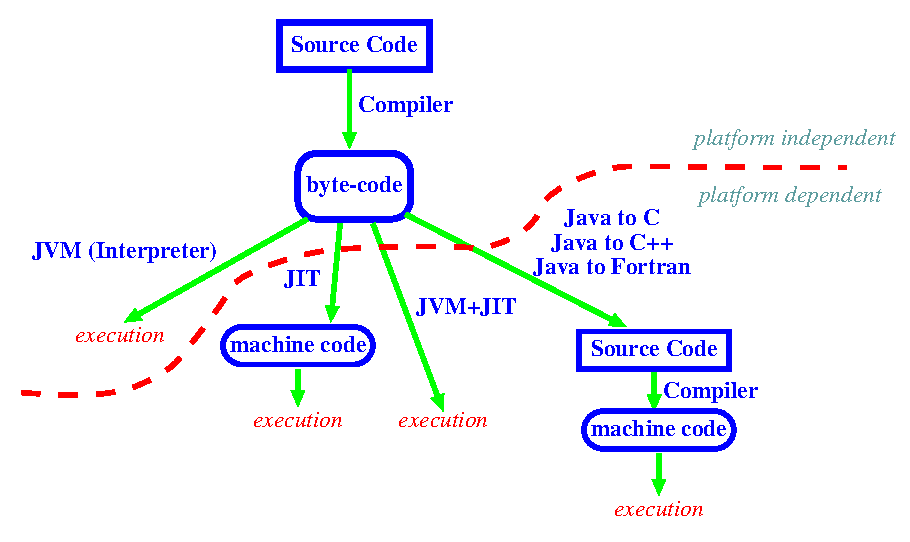
\includegraphics{Figures/Java_Overview.eps}
    \caption{Overview of the Java language execution model.}
    \label{fig:Java_Overview}
  \end{center}
\end{figure}

So for every platform, where a virtual machine is available,
you can execute the byte-code without any compatibility problems.
But the ``look and feel'' can be different, for example Java buttons
in Windows look different from buttons in X11/Motif using a UNIX
operating system. But if you use the new Swing components supplied
with the Java 2 standard or extend the Java 1.1 standard with the Swing
components, you can choose the appearance of the graphical look, which then
is the same across all platforms. So if you are using the new Java 2 standard
(JDK1.2), you should definitely use the new Swing components. If you
still use the AWT components (like we do here in this book), you should
keep in mind that the look (not the functionality) 
of the program can be different on different platforms. 
A big advantage of the Swing components is that they do not use any
native code, which the AWT components do.

The main reason for the wide availability of Java
is that SUN Microsystems distributes the Java Development Kit (JDK)
freely for a number of important platforms (Windows, Solaris/Linux,
other Unix systems). The JDK consists of a compiler (javac), a
debugger (jdb) and a virtual machine (java)\footnote{Actually there
are some more components like the javadoc command to create HTML
documentation or the jar tool to create zipped packages of
class files belonging together - see later on.}.

The JDK can be downloaded from the internet from the 
\href{http://www.javasoft.com}{JDK Javasoft link page}.
The newest version (as of the time of writing) is 1.2. 
Throughout the book,
we will use the Java 1.1 language version and the JDK 1.1.7,
because the Java 2 standard is not yet implemented in any JVM of the
web browsers available.

The only additional thing necessary to have a Java programming
environment is an text-editor to write the Java programs. For that
you should use your favorite editor, e.g. emacs or xemacs, which are
also freely available and have nice Java editing modes.

There is also a freely available IDE (Integrated Development 
Environment) called \href{http://www.freebuilder.org/}{FreeBuilder}.
This is a complete environment to write Java programs comfortably,
which is the first under the GNU license. It is still in alpha
development stage, but it already comprises a lot of features. Of
course, there are many commercial ones available, like SUN's Java Workshop
or Simplicity for Java (WWW ???).


Opposing to other languages, which use the ASCII character set, Java
uses the Unicode character set \href{http://unicode.org}{(Unicode WWW
Homepage)}. 
Unicode consists of characters represented
by 2 bytes instead of 1 byte like in the ASCII set. So you can not only
use 256 different characters (ASCII) but you can use all the 38885 different
characters available in the Unicode set (Version 2) for writing a Java program.
This means you can name your variables using for example Japanese or Greek
characters. Right from the beginning, Java is an international language.

Java is also case sensitive and doesn't need any special characters
to mark continuation lines. 

Comments are used just like in C and C++.
You can use either the /* \ldots */ syntax (borrowed from C) for
multi-line comments or the // syntax (borrowed from C++) for single
line comments. Additionally you can use /** \ldots */ for comments
to automatically generate a HTML documentation file for the class
defined in the file. We will see later on how this can be achieved.
 
There are also certain disadvantages, which should not be forgotten
to mention: The learning curve is certainly steeper for the beginner
for Java than for Matlab or even Fortran. This is of course due
to the full use of the object oriented approach used for all Java
programs. This clearly shows up, when we will introduce e.g. the
file and keyboard input/output capabilities of Java.
But in the long term learning Java definitly pays off. 

A second point to note is, that for scientists a big concern are always
complex numbers. They are currently not supported as primitive types as 
in Fortran for example, but there are (standardized) packages, which
add complex number support to Java (e.g. JNL). 


\subsection{The ``HelloWorld'' Program -- Applications and Applets}
\label{sec:HelloWorld}
Now let us start with the traditional ``Hello World'' program written
in Java.

\subsubsection{Application}

\inputlisting{Listings_Java/HelloWorld_Application.java}
You have to save the program in a file called 
\verb|HelloWorld_Application.java|.
To execute the above example you have to type in the commando line the
following:
\begin{itemize}
\item Compiler: \verb/javac HelloWorld_Application.java/  \\
  $\Longrightarrow$ produces HelloWorld\_Application.class 
  in the same directory.
\item JVM:  \verb/java HelloWorld_Application/
\item Output on screen: \verb<Hello World !<
\end{itemize}
Let us now try to understand the above code. The program consists of
three lines. 

In the first line the program declares 
with the help of the \texttt{class} statement a class called 
\verb|HelloWorld_Application|. 
The identifier following the \texttt{class} statement is
the name by which the class will be referenced. Each Java program
is a class. The curly bracket appearing after the class name
\verb|HelloWorld_Application| introduces the following class member. 


In the second line the \verb|main| method is introduced. The main
method is declared \verb|void| because the method does not return a
value. The main method is executed when you run the class as an
application. The only parameter, the argument
of the main method, is an array of String object.

In the third line the method \verb|println()| of the system class 
\verb|out|
is invoked. This method simply prints a string and terminates with a 
new--line command. Alternatively you could use the 
\verb|System.out.print()| method, which does the same, but does
not print a newline at the end. 

You have just written and executed your first application in
Java. Please, do not worry if you do not understand everything. You are
not expected to understand everything at this stage.

If you are using Emacs/XEamcs and JDE you could have started Emacs and
then just used the ``JDE New'' method in the ``Files'' menu. Then you
have to type the \verb|System.out.println()| code, which could
again be accomplished by using the \verb|Generate| menu in the
JDE menu. To compile
use the ``compile'' command in the ``JDE'' menu and similar
the ``run'' command in the same menu. This saves you a lot of keystrokes. 

\subsubsection{Applet}
\label{sec:Applet}

Java offers another possibility to execute code, so called Applets.
In contrast to the stand--alone Java application which starts at
\verb!main! and runs until it is completed, the applet is a kind of
sub--program which runs under the control of some other program.
Usually, applets are (small) Java programs, which are started by a 
server program,
e.g. a WWW browser like Netscape Navigator\footnote{You need at least 
version 4.06 or patches for earlier versions to use all features of Java 1.1}, 
the Internet Explorer\footnote{Seems to run Java 1.1 programs since
version 4, but does not conform to the Java standards.}(Don't),
HotJava or the appletviewer\footnote{included with the JDK.}.

In the case of an applet, you have a browser loading a HTML 
(Hyper Text Markup Language) file. This HTML file contains
markups, which tell the browser what applet to load and
where to find the applet (see figure \ref{fig:HTMLOverview}). 
\begin{figure}[htbp]
  \begin{center}
    \includegraphics[width=\textwidth]{Figures/HTMLOverview.eps}
    \caption{An HTML file gets loaded into the browser. The browser itself formats the text and if it finds an applet mark, it starts the applet.}
    \label{fig:HTMLOverview}
  \end{center}
\end{figure}
You should note that HTML is not a programming language, but
it is a mark-up language to produce a text with additional
``commands'' for the meaning of the text parts. It does also
not give any details about the formatting or layout of the
text. To start an applet HTML has some special marks, which we
will see in a moment.  

The big difference between an applet and an application is that
applets are not allowed to do certain things. For example applets
do not have access to local file systems, so it is not possible
to save data on the file system from an applet. It is also not
possible for an applet to issue a print command, the process of
printing has to be initiated by the server (browser). 
And an applet is not allowed to do time consuming tasks like
long computations. This has to be kept in mind, when writing
applets.

You can actually have applets accessing the local file system by using
``signed applets''. These are applets having a signature coming
with them (in the JDK you use \verb|javakey| for that purpose), 
which is checked by the server before the execution. So
if you have signed your own applet and tell your browser to accept 
all applets signed with your signature, you can use file commands
inside your applets (see \cite[page 142]{javanutshell}).

The ``Hello World'' example written as an applet has the following form:
\inputlisting{Listings_Java/HelloWorld_Applet.java}

Applets have to be derived from the applet class
\verb|java.applet.Applet|, which include the principal facilities of
the Abstract Windowing Toolkit (AWT) and the interface with X/Motif on
Unix, Windows on PC, and Mac-OS on Macintosh platforms.
As you can see there is no main method in an applet. Instead if an applet
is started by a server, the init() method is executed first. There is also
a start() (stop()) method, which is executed if the applet becomes
visible (disappears) in the server window (e.g. by scrolling in the
Netscape Navigator window).

Many methods are available to set up the display in an assigned applet area.
The paint() method appearing in the ``Hello World'' applet is
responsible for the visual part of the applet. It uses a canvas
(drawing area) with a size defined by the calling HTML file. In our case
this HTML file could look like:
\inputlisting{Listings_Java/call_HelloWorld_Applet.html}
The code parameter given in the HTML file defines the name of the applet
to be run. Because there is no init() and no start() method in our
example, the paint() method gets executed by the browser (or appletviewer).
The size of the canvas has to be given in pixels explicitly in the
HTML file.

To run the applet you can either type
\begin{itemize}
\item \verb|appletviewer  call_HelloWorld_Applet.html| or
\item use the following URL in the browser: \\
        \verb|PATH_TO_CLASS_AND_HTML_FILE/call_HelloWorld_Applet.html| \\
        e.g. \verb|/home/user/java/call_HelloWorld_Applet.html|
\end{itemize}

The question arising now, when to use an application and when to use
an applet, is difficult to answer. In the following chapters we will 
decide for each program
separately, which way to go. Time consuming calculations should
definitely be written as an application, small programs can be
written as an applet of course.

In Java 1.1 a new package (see later) was introduced, which allows
so called ``trusted applets''. These are specially signed libraries,
which are signed with a key by a person you trust. Only if the
signature is valid and you trust that person, the ``trusted applet''
has access to the local files system -- basically it can do everything
an application could do on your machine. This is already implemented with
the appletviewer, in different ``servers'' it might work or not. In the
future this will be extended to a more extensive set of rules for the
allowed methods of an applet.

\paragraph{Documenting Java Programs -- javadoc}
A last remark concerns the documentation for the programs. We have
learned, that we can include documentation comments using 
\verb|/** .... */|. These comments are processed by using the
\verb|javadoc| command from the JDK. If you run the javadoc command as: 
\begin{sverbatim}
  javadoc HelloWorld_Application.java HelloWorld_Applet.java  
\end{sverbatim}
you get some HTML files: packages.html, tree.html, AllNames.html,
HelloWorld\_Applet.html, HelloWorld\_Application.html. All these
files describe the written classes. The tree.html file gives a tree
showing the relatives of the class. The package.html gives the
package structure (not used here). The most important file is the
AllNames.html, which is an index of all written programs in this package
(for an introduction to packages see later).

You can even include special predefined strings to supply the
author and many more informations to the javadoc command, either
for a class or a method, whereas the documentations for the method
can also be supplied for a class:
\begin{lstlisting}{}
  /**
      @author Peter Biechele
      @version 1.0
  */
  .. class ... { }

  /** 
      @see <a class name>
      @see <class name>#<method name>

      @param  a b c
      @return d
      @exception  none
  */
  .. method ... { }
\end{lstlisting}

This of course gives us the opportunity to write our 
explanations/documentation
betweeen the \verb|/** .... */| commands using HTML constructs like
\verb|<hr>| for a horizontal rule or others - try it. 
Because this code gets directly included in the HTML files produced by
the \verb|javadoc| command, you can have nicley formatted documentation.
But you should avoid using \verb|<h1>| to \verb|<h6>| -- the heading 
commands -- because javadoc uses them for its own structure.

If you load AllNames.html into a browser, you get the HTML file shown
in figure \ref{fig:javadoc1}.
\begin{figure}[htbp]
  \begin{center}
    \leavevmode
 \includegraphics[width=8cm]{Figures/AllNames.eps} 
    \caption{The output of the \texttt{javadoc} command from the JDK 1.1.}
    \label{fig:javadoc1}
  \end{center}
\end{figure}
Now you can click on the link HelloWorld\_Applet and you get the
documentation for that class and analogous for the HelloWorld\_Application
class (see figure \ref{fig:javadoc2}).
\begin{figure}[htbp]
  \begin{center}
    \leavevmode
  \includegraphics[width=6cm]{Figures/HelloWorld_Applet.eps}
  \includegraphics[width=6cm]{Figures/HelloWorld_Application.eps}
    \caption{The output of the \texttt{javadoc} command from the JDK 1.1.}
    \label{fig:javadoc2}
  \end{center}
\end{figure}
The missing graphics on the right of figure \ref{fig:javadoc2} 
are available in the Java documentation of the
JDK and just has to be copied into a subdirectory  
of the HTML directoryc called \verb|images| . 
Then it looks like the figure on the left.

The javadoc command of the JDK 1.2 produces much nicer pages which
look like in figure \ref{fig:Java2HTMLDoc}. There are no separate 
gif pictures
needed anymore and the structure of the classes is represented
much better.
\begin{figure}[htbp]
  \begin{center}
    \includegraphics[width=7cm]{Figures/HelloWorldApplet2.eps}
    \includegraphics[width=5.5cm]{Figures/HelloWorldApplication2.eps}
    \caption{The output of the \texttt{javadoc} command from the JDK 1.2.}
    \label{fig:Java2HTMLDoc}
  \end{center}
\end{figure}

%%%%%%%%%%%%%%%%%%%%%%%%%%%%%%%%%%%%%%%%%%%%%%%%%%%%%%%%
\subsection{Variables}
\label{sec:Variables}

Essentially, Java distinguishes between two types of variables,
primitive data types and reference data types.
\subsubsection{Primitive data types}
\label{sec:primitive_data_types}
We already mentioned that in Java each variable or expression has a
definite type and that each type has identical size and behaviour on
all Java implementations.  Java has built in primitive data types
to support integer, floating--point, boolean, and character values.
The primitive data types of Java for integers, floating--points,
characters and boolean variables are listed in table
\ref{table:primitivedata}.
\begin{table}[htbp]
\label{table:primitivedata}
\begin{center}
\begin{tabular}{l|l|l|l|l}
Type & Contains & Default & Size & Min \\
     &          &         &      & Max \\ \hline \hline
byte  & signed integer & 0 & 8bits & -128  \\
&&& & 127    \\ \hline
short & signed integer & 0 & 16 bit &-32768 \\
&&& & 32767 \\ \hline
int &   signed integer & 0 & 32 bits&-2147483648 \\
&&& &2147483647 \\ \hline
long & signed integer & 0 & 64 bits &-9223372036854775808\\
&&& &9223372036854775807\\ \hline
float & floating--point & 0.0 & 32 bits &$\pm$1.40239846E-45\\
&&& &$\pm$3.40282347E+38\\ \hline
double & floating--point & 0.0 & 64 bits &$\pm$4.94065645841246544E-324\\
&&& &$\pm$1.79769313486231570E+308\\ \hline
boolean & true or false      &  false & 1 bit&\\
&&&       &  \\ \hline
char  & Unicode character & $\backslash$u0000 & 16 bits & $\backslash$u0000 \\
&&& &$\backslash$uFFFF   \\ \hline
\end{tabular}
\end{center}
\caption{Primitive data types in Java. The byte and char data types have
  been introduced in Java 1.1 and in Java 2 there was a void type added.}
\end{table}


The following comments have to be made. In a Java program every
variable must have a type that precedes its name when the variable is
declared. For example the integer i may be declared as
\begin{verbatim}
int i;
\end{verbatim}
and integer/long values can be expressed as
\begin{verbatim}
int i = 123;    long l = 1234567889L;   long l2 = 123456789l;
\end{verbatim}

Char values represent characters. They appear in Java between single
quotes, e.g.
\begin{verbatim}
char c = 'C';
\end{verbatim}
A Unicode character is represented by the Unicode escape sequence
$\backslash$uxxxx, where xxxx is a sequence of four hexadecimal digits.


Float and double types have special values that may be the result of
certain floating-point operations. For example in the java.lang.Float
and java.lang.Double classes the special values
\verb|POSITIVE_INFINITY|, \verb|NEGATIVE_INFINITY|, and 
\verb|NaN| (not-a-number) are
defined.

Floating point numbers are expressed as e.g.
\begin{verbatim}
13.       1.3e1        .13E2 
\end{verbatim}
and are considered to be constants of type \verb|double| 
unless they are specified with \verb|f| or \verb|F|, which makes them
then \verb|float| constants.

In Java strings are not of primitive type and they are not an
array of chars like in C. Java provides a String
class to deal with sequences of character data. The java string
class provides methods to operate on String objects.

All variables in Java are initialized automatically, as soon as they
are declared. All primitive types get initialized to zero, the boolean type
to false and all objects (remember they are references) are initialized
to \verb|null|. So there is no ambiguity like in other languages, if
a variable has a defined value at certain points of the program. 
Although Java forces you to include sometimes a statement to
initialize variables, just to make easier to read source code.
We will see an example for this later on, when we discuss loops
and calculate averages of sequences of numbers.

\subsubsection{Reference data types}
\label{sec:Reference_data_types}

All non-primitive data types in Java are objects and arrays. They are
called also ``reference types'' because they are handled by
reference. For example you may pass the address of an object, which is
stored in a variable, to a method. In contrast, primitive types are
always passed by value.


%%%%%%%%%%%%%%%%%%%%%%%%%%%%%%%%%%%%%%%%%%%%
\subsection{Casting and Type Conversions (Wrapper Classes)}

Java uses a clear strategy to convert the primitive data types to 
other primitive ones. In a calculation Java always converts (casts)
the less precise type to a more precise one. So if you multiply an
integer and a float value, it converts automatically the integer to
a float and then multiplies both values. If you want to convert
a value explicitly you can use the cast operators (like in C and C++).
Just write the primitive type in round brackets in front of the value to
be converted, e.g. \verb|result=(double)a*b| casts \verb|a| to 
a double value and
then multiplies it with \verb|b|, assigning the result to \verb|result|.
You can also use the wrapper classes to be discussed below, but
it is much more complex and should be avoided.

A common problem is to convert from strings to primitive types and
vice versa. Because strings are objects and not primitive types, we
need a method for the conversion. For that reason Java has so called
wrapper classes, subclasses of the \verb|java.lang.Number| class 
for all primitive datatypes. 
These classes provide all the necessary methods for all types of
conversion. 

The static \verb|.valueOf(String s)| method always converts a string
to the corresponding wrapper class of a primitive type, e.g. 
\begin{lstlisting}{}
        double a;
        String text="+1.234";

        Double D = Double.valueOf(text);
        a = D.doubleValue();

        a=Double.valueOf(text).doubleValue();
\end{lstlisting}
The fourth line converts the string to the \verb|Double| class and in the
fifth line 
the \verb|doubleValue()| method converts the Double wrapper class 
to a double primitive type. The last line shows how to do it in
one line.
For the other types you just have to substitute float or int 
for double, i.e., \verb|floatValue()|, \verb|intValue()| and the
corresponding wrapper class (\verb|Integer| for \verb|Double|, etc.).
 
Another (easier) method, 
later used in the \verb|ParamApplet.java| program is, e.g.,
the \verb|Integer.parseInt(String s)| method, which gives back a primitive
type integer instead of the wrapper class like \verb|valueOf(String s)|.
For other conversions you can use the \verb|Long.parseLong(String s)| or the
\verb|Long.parseByte(String s)| method.

These methods  simplify the conversion a little bit. For the example, see
\verb|ParamApplet.java| in line 11. But this method is only 
available to Integer, Long and Byte wrapper classes, NOT for
Float and Double as of Java 1.1. Fortunately they are included in the
Java 2 specification.
In the Java 1.1 case you have to use the \verb|valueOf(String s)| and
\verb|doubleValue(String s)|, \verb|floatValue(String s)| methods.

To convert a double value to a string you have to use the \verb|toString(dobule d)|
method, which is available for all primitive data types.
For example, two ways of doing it are:
\begin{lstlisting}{}
  double d = 3.1234;
  String s1 = Double.toString(d);    <------ most easy way
  String s2 = (new Double(d)).toString();
\end{lstlisting} 



%%%%%%%%%%%%%%%%%%%%%%%%%%%%%%%%%%%%%%%%%%
\subsection{Packages and Import Statements}
\subsubsection{Packages}
Because Java was designed to be able to load code distributed
over the whole internet dynamically, you have to avoid name conflicts
between the programs (classes). The Java solution 
for an Internet--wide unique naming scheme is to put
every class in a \emph{package}. A package  is a group of related
and possibly cooperating classes. The naming scheme is based on the
internet domain name of the organization at which the package is developed.

The name of the package is given
at the beginning of a file before the actual program (class)
definition starts. So for example if we put the statement
\begin{quotation}
  \verb/ package de.freiburg.simulation; / 
\end{quotation}
at the beginning of the ``Hello World'' application, we can compile
the application with \verb/javac HelloWorld_Application.java / like before.
But to run the application we have to use
\begin{quotation}
  \verb/ java de.freiburg.simulation.HelloWorld_Application / . 
\end{quotation}
You are wondering why the program does not start? It cannot, because
there is one more thing to know. Java is looking for programs (classes)
in the directory structure given by the class name. So
for the example above you have to put the \verb/HelloWorld_Application.class/ file
in the directory \verb|de/freiburg/simulation/| and issue the command
in the directory, where the directory tree starts.

You could also use an environment variable called \verb|CLASSPATH|. It
describes the directories to search for the class files. So if the
\verb|CLASSPATH|-variable includes \verb|/home/user/java| you can
start the above example in this directory, if the class is in the 
subdirectory  \verb|de/freiburg/simulation/|. It has to be noted that
the entries in a \verb|CLASSPATH| specification may also be ZIP files
that contain these classes. On Unix systems the directories in a
\verb|CLASSPATH| specification are separated by `` :'' ( on Windows systems
by ``;'').


All the standard commands (classes) of Java are stored in a central jar
file, which is additionally packed to save disk space. These classes
are always searched, no matter the \verb|CLASSPATH|-variable is set to.

If you are not using the package command at all, Java uses the empty 
package. This means you can put your programs in the current directory.
This is not recommended for medium to complex programs, but for
test purposes and very small programs this is very convenient.

\subsubsection{The jar Tool}
If you have written a lot of small classes, which all work together
(called a project), you
can put them all inside a ``jar'' file and give the jar file
to friends instead of the whole bunch of small class files.
A jar file is just an archive created by the \verb|jar| program 
coming with the JDK. It works like the well-known UNIX \verb|tar|
command. This is actually a very nice method for packaging
applets on the internet, because the jar command also compresses
its contents. 

For example to view the contents of a jar file you can issue the command
\verb|jar tvf lava.jar| (the Lava Rocks jar file). Some of the
available options used with jar are given in table \ref{tab:JarOptions}.
\begin{table}[htbp]
  \begin{center}
    \begin{tabular}{cp{0.7\textwidth}}
      Option & Description \\\hline
      c & create jar file\\
      t & table of contents of jar file\\
      x & extract files from jar archive\\
      f & name of jar file comes as first argument after options (the
          default is the standard input/output) \\
      v & verbose output \\
      O & do not compress (used for jars residing in the CLASSPATH)\\
    \end{tabular}
    \caption{Options of the jar command. The jar tool is included in the JDK.}
    \label{tab:JarOptions}
  \end{center}
\end{table}
Jar files are portable from one platform to the other, but as you can 
see jar is not as powerful as the tar command in UNIX.


\subsubsection{Import statement}
Before learning more about the syntax of Java, we have to explain another
statement appearing in the part of any Java program before the actual
definition of the class: the \verb|import|-statement. With \verb|import|
you can make classes available, so you don't have to use the fully
qualified name to the class. So if you would like to
use the HelloWorld class from above in your programs, you could either
type \verb|de.freiburg.simulation.HelloWorld()| in your program
or you can use
\begin{sverbatim}
import de.freiburg.simulation.*;
....
   HelloWorld();
\end{sverbatim}
to import all classes in the \verb|de.freiburg.simulation| class.
You can also use:
\begin{sverbatim}
import de.freiburg.simulation.HelloWorld;
....
   HelloWorld();
\end{sverbatim}
if you just want to import one special class.

We have already made use of the \verb|import|-statement in the ``Hello World'' 
applet. There we have imported the \verb|java.applet|-class, which
defines applets and their behaviour, and the \verb|java.awt|-class, which
will be explained later.
 
There is one class, which is always imported without any import statement:
the \verb|java.lang.*| classes. This is the fundamental class of Java and it is
implicitly imported for all Java programs, so you do not have to specify
it. For example the System class is in \verb|java.lang|, that is why
we did not have to use an import statement in the ``Hello World''
application.  


\subsection{Compiling Projects}
If you write a program consisting of many classes and files, you
may think that this is a lot of work to compile all of them. Or if
you are used to writing code in other languages, you might think
of using tools for checking if a program has to be recompiled, if you make
changes to some files. One of these tools might be the famous ``make''
utility. But fortunately this is not needed for JKava, because
the JDK developers (or to be precise the Java standard) already
takes care of these problems. 

You have to arrange your code in the different classes according to 
certain rules (packages). So the directory structure is already a
nice tree structure of your project. If you then want to compile
the whole project, but only the files which have changed\footnote{Notice
that there is no dependance of classes on others classes in the
sense of recompilation. Java does dynamical run-time linking and no static 
linking at the end of the compilation process as in all other languages.}
should be recompiled, you issue the
command \verb|javac -depend -d base_directory main.java|. Then
the Java compiler takes care of all ``dependencies''.   

%%%%%%%%%%%%%%%%%%%%%%%%%%%%%%%%%%%%%%%%%%
\subsection{Simple Arithmetics, Conditional Statements and Loops}
\label{sec:Loops}

\subsubsection{Simple arithmetics}
As we already mentioned Java  supports almost all of the standard
C operators. The arithmetic operators that operate on numerical types
are 
\begin{center}
\begin{tabular}{ll}
$+$ & addition \\
$-$ & subtraction                 \\
$*$ & multiplication \\
$/$ & division \\
\% & remainder
\end{tabular}
\end{center}
The $+$ operator can also be used to concatenate strings, as we will
see later in an example in section \ref{sec:Parameter}.
There is no power operator like \verb|**| in FORTRAN or \verb|^| like in many
different programs like TeX/LaTeX. In Java like in C/C++ you have to use
a special mathematical function/method 
(\verb|Math.pow()|, see in a later section).

It is important to remark, that in Java integer division truncates
toward zero (7/2=3, -7/2=-3 and -7/-2=3).

Java has two special operators for increment $++$ and decrement $--$. The 
expression \verb|i++| is equivalent to \verb|i=i+1| except that
\verb|i| is evaluated only once. They can be used as pre- and post-operators,
depending on the position of the symbols, e.g. \verb|i++| or \verb|++i|.
This does not make a difference, if you just have these statements
alone, but in some complex expressions this might make a difference.
The postfix (prefix) version of the operator ++ evaluates  the value
of the operand before (after) the increment operation.
For example \verb|i = j++| means setting i to j and then increment j by one.
But \verb|i = ++j| means setting i to j+1.

There is no operator for calculating powers, instead you have to use
(like in C) the \verb|Math.pow()| method of the \verb|Math| class.
The \verb|^| operator, used sometimes for the power, is the exclusive
or (XOR) operation in Java (either in the logical or the boolean sense). 
So do not confuse this. 

Java supports also a standard set of relational and logical operators,
which all yield boolean values. They are listed below

\begin{center}
\begin{tabular}{ll}
$>$  & greater than \\
$>=$ & greater than or equal to \\
$<$  & less then \\
$<=$ & less than or equal to \\
$==$ & equal to \\
$!=$ & not equal to
\end{tabular}
\end{center}


The conditional operators
\begin{center}
\begin{tabular}{ll}
\& \& & conditional AND      \\
$\mid\mid$ & conditional OR
\end{tabular}
\end{center}
operate on  boolean expressions only.

Java has also bitwise operators which operate on integers and on
boolean types. They allow to perform bit manipulation on data.
\begin{center}
\begin{tabular}{ll}
\& & and \\
$\mid$ & or \\
$\tilde{}$ & not \\
$<<$ &  shifts bits left filling with zero bits on the right \\
$>>$ & shifts bits right filling with the highest sign bit on the
           left--hand side \\
$ >>>$ & shifts bits right filling with zero bits on the left--hand side 
\end{tabular}
\end{center}

Last not least we have to mention the fundamental assignment operator
$=$. It may be used in combination with other operators, e.g., $+=$
means is incremented by.


\subsubsection{Loops}
\paragraph{for Loops}
For our forthcoming applications the most important control statement
is the \verb|for| statement. It is used to loop over a range of values
from the beginning to the end. Its syntax is
\begin{sverbatim}
for (init_expressions; boolean_expr; incr_expressions) {
    statements
}
\end{sverbatim}
where \verb|init_expressions| denotes the initial value of the iterated
variable, \verb|incr_expressions| denotes the increment of the iterated
variable. For both you can specify more than one expression separated
by commas (as in C). This is the only place, where you can use these comma
separated lists. The variables used in the for statement can be 
integer (long) or float (double) values. 

At the beginning of the \verb|for| loop the boolean expression
\verb|boolean_expr| is evaluated. If its value is found to be 
\verb|true| the statement is executed repeatedly with increment
\verb|incr_expr| until the value of the boolean expression is found to
be \verb|false|.

As an example demonstrating the use of
\verb|for| loops we want to write a program to calculate the mean of
a given number of random numbers. One possible implementation
could look like this:
\inputlisting{Listings_Java/DataMean.java}

Here we used the class \verb|java.util.Random| which allows for
the creation of random numbers. If we don't supply a seed, as is the
case here, it just uses the time to initialize the generator. The
initialization takes place in line 10, where a new generator is created.
You can check this by running the application more than once and comparing
the means -- they should not be the same. 

The \verb|next.Double()| method returns a new random number of type
double (for a float use \verb|rand.nextFloat()|). You can also create normally 
distributed random numbers with the \verb|nextGaussian()| method of
the \verb|Random| class.
The remaining parts of the program should be self explaining. You can of
course use any expression (e.g. \verb|d=d*u+2|) 
in the last part of the for statement, not only
the \verb|++| operator, which is obviously used most often. 

\paragraph{Byte-Code of a class file}
Using the \verb|DataMean()| program, we want to show the bytecode
produced by the Java compiler. In the first line you can see the
command to use (\verb|javap|) and below the output:
\begin{scriptsize}
\begin{verbatim}
Command_Line>>> javap -c DataMean

Compiled from DataMean.java
public synchronized class DataMean extends java.lang.Object
    /* ACC_SUPER bit set */
{
    public static void main(java.lang.String[]);
    public DataMean();
}

Method void main(java.lang.String[])
   0 sipush 10000
   3 istore_3
   4 new #10 <Class java.util.Random>
   7 dup
   8 invokespecial #12 <Method java.util.Random()>
  11 astore_1
  12 dconst_0
  13 dstore 4
  15 iconst_1
  16 istore_2
  17 goto 32
  20 dload 4
  22 aload_1
  23 invokevirtual #17 <Method double nextDouble()>
  26 dadd
  27 dstore 4
  29 iinc 2 1
  32 iload_2
  33 iload_3
  34 if_icmplt 20
  37 dload 4
  39 iload_3
  40 i2d      
  41 ddiv
  42 dstore 4
  44 getstatic #18 <Field java.io.PrintStream out>
  47 new #8 <Class java.lang.StringBuffer>
  50 dup
  51 ldc #2 <String " The mean of ">
  53 invokespecial #13 <Method java.lang.StringBuffer(java.lang.String)>
  56 iload_3
  57 invokevirtual #15 <Method java.lang.StringBuffer append(int)>
  60 ldc #4 <String " random numbers
">
  62 invokevirtual #16 <Method java.lang.StringBuffer append(java.lang.String)>
  65 ldc #3 <String " between 0 and 1 is ">
  67 invokevirtual #16 <Method java.lang.StringBuffer append(java.lang.String)>
  70 dload 4
  72 invokevirtual #14 <Method java.lang.StringBuffer append(double)>
  75 ldc #1 <String " !">
  77 invokevirtual #16 <Method java.lang.StringBuffer append(java.lang.String)>
  80 invokevirtual #20 <Method java.lang.String toString()>
  83 invokevirtual #19 <Method void println(java.lang.String)>
  86 return

Method DataMean()
   0 aload_0
   1 invokespecial #11 <Method java.lang.Object()>
   4 return
\end{verbatim}
\end{scriptsize}

\paragraph{while and do--while}
Java offers also the possibility to use other loop constructs, the
\verb|while| and the \verb|do-while| loop. There syntax is
\begin{verbatim}
while (boolean_expression)
 statement
\end{verbatim}
and
\begin{verbatim}
do
  statement
while (boolean_expression)
\end{verbatim}
It is important to observe that in the first construct the boolean
expression is evaluated \textit{before} the statement is executed, while in
the second construct the boolean expression is evaluated \textit{after} the
statement has been performed!

In order to give an example we write down an equivalent code using
the
\verb|while| statement of the \verb|for| loop of the
\verb|DataMean.java| program. Lines 13 to 15 have to be replaced by
\begin{verbatim}
int i;
while(i<N){
  mean += rand.nextDouble();
  i++;
}
\end{verbatim}

\subsubsection{Conditional Statements}
\paragraph{if-else}
The \verb|if| statement is the fundamental form of conditional control
of flow. It allows to choose, whether the statements that follow it are
executed or not. Its syntax in Java is
\begin{verbatim}
if (boolean_expression) {
   statement1
}
else if (boolean_expression) {
   statement2
}
else {
   statement3
}
\end{verbatim}
First, the boolean expression is executed. If the value is \verb|true|
then \verb|statement1| is performed, otherwise if there is the
optional \verb|else| statement \verb|statement2| is executed. Of
course, \verb|if-else| constructions can be nested, i.e., an
\verb|if-else| conditional control flow, can be placed within another
\verb|if-else| statement.

\paragraph{The conditional operator ?} The conditional operator ?
provides a single expression yielding one of two alterantives depending on
a boolean expression. To demonstrate its use we write down an
\verb|if/else| Java code first and translate it into an equivalent  ? 
construction. The \verb|if/else| code reads

\begin{verbatim}
if (a<b) 
  x=1.0;
else
  x=2.0;
\end{verbatim}
The equivalent construction with the conditional operator ? is more
compact
\begin{verbatim}
x= (a<b ? 1.0 : 2.0);
\end{verbatim}
The meaning of the different expressions in the above stement should
be obvious.


\paragraph{(labelled) break and continue -- goto}
We already remarked that Java does not have a \verb|goto| instruction
to transfer control to an arbitrary statement in a method. To handle
with situations where other languages have a \verb|goto| Java provides
the labelled \verb|break| and \verb|continue| statements. Labels are
typically used in blocks and loops and precede statements
\begin{verbatim}
label: statement
\end{verbatim}
The \verb|break| statement is used to exit from a block, e.g. to break
out of a loop. E.g., an unlabeled \verb|break| terminates the innermost
\verb|for|, \verb|while| or \verb|do|.

The \verb|continue| statement is used only within loops. It skips to
the end of the loops body and evaluates the boolean expression that
controls the loop. The \verb|return| statement terminates execution of
a method and returns to the invoker. If a method returns no value you
have to use
\begin{verbatim}
return;
\end{verbatim}
if the method has a return type, the \verb|return| must include an
expression for a returned type. You can use as many return statements 
as you like, but only one is executed each time the method gets called.

\paragraph{recursive programming}
As in most other languages, recursive programming is allowed, although
it should be avoided. First because of the clarity of the code
and second it has low performance and larger memory consumption. 
Therefore we do not see any reason to show an example, just
avoid using recursive algorithms.

\paragraph{switch/case}

Another central flow structure is the \verb|switch| statement. It
evaluates an integer expression whose value is used to find an
appropriate \verb|case| label among those listed inside the following
block. The \verb|switch| statement may be used to replace nested \verb|if-else|
statements that determine what is the output for each number. The
\verb|switch| statement works only if the value being tested is a
primitive integral type and when the value is tested against constant
values. the basic syntax of the \verb|switch| statement is
\begin{verbatim}
switch(expression) {
    statements
}
\end{verbatim}
After evaluating the expression, the switch statement executes
certain code within the block depending on the integral value of the
expression. This information is indicated by the integer label following
the \verb|case:| statement. If there is no \verb|case:| label that
matches the value of the expression, the \verb|swich| command executes
the code following \verb|default:|, if there is one. Otherwise,
\verb|switch| does nothing.

An example of the use of the \verb|switch| statement is found in the
simple program \verb|DiceGame.java| 

\inputlisting{Listings_Java/DiceGame.java}

Again we want to stress that only an integer, long, char or byte type
is possible in the switch statement (no double or float). And the
case expressions have to be integral values and not any boolean
expressions like \verb|i>2|. 

%%%%%%%%%%%%%%%%%%%%%%%%%%%%%%%%%%%%%%%%%%%

\subsection{Arrays and Matrices}
\label{sec:Arrays}

Before discussing the notion of classes and objects, we want to introduce
another reference type: the array. Arrays are actually objects
(see \ref{sec:objectoriented}), but
Java provides many special commands for arrays, which makes them a 
little bit special.

The first question is how to create arrays and how to destroy them.
The destruction is easy to explain: it is done automatically
by the garbage collector (like for all objects). This is different to
other languages like C, C++ and Fortran 90, where you explicitly
have to destroy (free) the allocated memory. 
\begin{table}[htbp]
  \begin{center}
    \begin{tabular}{c|c|c}
      C & C++ & Java \\\hline
      malloc & new & new \\
      free & dispose & -- \\
      \multicolumn{2}{c}{Pointer} & References + Garbage Collector \\
      \multicolumn{2}{c}{Pointer arithmetic possible}& there is no 
                                                    reference arithmetic \\
    \end{tabular}
    \caption{A comparison of the different memory allocation commands in different languages.}
    \label{tab:MemoryAllocation}
  \end{center}
\end{table}
To create an array you have to use the \verb|new| keyword used for
creating (instantiating) objects. So to create a one dimensional
array, called \verb|intarray|, with 10 elements you use:
\begin{verbatim}
        int intarray[] = new int[10];
\end{verbatim}
This also sets all the elements to zero. But this is only true for 
primitive types. Arrays of reference types (objects) are created the
same way, but the elements consist of references to the elements. The
elements themselves are NOT initialized and have to be created too.
An example for this is a two dimensional array as we will see soon.

Indices of arrays in Java start with zero as in C and not with 1
as in Fortran. No negative indices are allowed in Java. The length
of an array (meaning the number of elements) is always given
by the \verb|.length| field. For the array above you get the number
of elements by using \verb|intarray.length|. We have already met
this notation when we discussed the command line parameters.

You can also create the array and initialize it right away by using
(also in Java 1.0):
\begin{verbatim}
  int intarray[] = {1, 2, 3, 4, 5, 6, 7, 8, 9, 10};
  int[] intarray = {1, 2, 3, 4, 5, 6, 7, 8, 9, 10};
\end{verbatim}
or one step further, create an array of objects (here strings) and
create the elements in the same step:
\begin{verbatim}
  String stringarray[] = {"a","b","c","d","e","f","g"};
\end{verbatim}
In Java you can even put the brackets behind the type instead of the
variable name (not possible in C). So it does not matter if you
write \verb|int intarray[];| or \verb|int[] intarray;|.

In Java 1.1 you can also use \emph{anonymous arrays}:
\begin{verbatim}
  String[] texts;
  texts = new String[] {"a","b","c","d","e","f","g"};
  System.out.println(new char[] {'h','e','l','l','o'});
\end{verbatim}
So you can create and initialize arrays without even using a variable.

Multidimensional arrays are also supported. Just like in C they are
arrays of arrays. For example
\begin{verbatim}
  double matrix[][] = new double[10][10]; 
\end{verbatim}
creates a 10 by 10 matrix, called \verb|matrix|, 
meaning that you have created 10 arrays
of type \verb|double[10]|. An important point to make is that you
do not have to specify all dimensions at once. You can for example
create a triangular matrix by submitting:
\begin{verbatim}
  double matrix[][] = new double[10][];
  for (int i=0; i<10; i++) {
         matrix[i] = new double[i+1];
  } 
\end{verbatim}
To access multidimensional arrays you can also use one dimensional
array syntax (as in C). If you have a two dimensional array 
you can access the element [i,j] by accessing the element [i+j*columns]. 

Now let's look at an example using arrays. We have rewritten the program
\verb|DataMean| above to calculate the average of random 
numbers by using arrays.

\loadlisting{DataMeanArray.java}{Listings_Java/DataMeanArray.java}

Here we first declare a double array called \verb|RandomNumber| and
create it in Line 13. Then we store the random numbers in the array
and afterwards calculate the mean.
The last important point to address is the copying of arrays. 
You can not just write
\begin{verbatim}
  int[] array1 = {1,2,3,4,5};
  int[] array2;
  array2 = array1;          // WRONG ! - ERROR ! 
\end{verbatim}
This would only copy the reference of the array1 object to the array2
object, not the values, the memory address is the same. 
To copy the values of arrays you have to use the 
\verb|arraycopy()| method of the java.lang.System class. 
So to copy an array in the above example, you have to write:
\begin{verbatim}
  System.arraycopy(array1,0,array2,0,array1.length);
\end{verbatim}
This copies all elements of array1 to array2 staring from element 0. 
The remaining parts of array2 are not created!

\subsection{Arrays in Java 2}
A new class \verb|Arrays| in the \verb|java.util| package has been
introduced in Java 2, which is of great interest not only to scientific
programmers. It includes methods for sorting arrays of arbitrary
type using a modified version of the Quicksort\footnote{This is
a sorting algorithm, which is very versatile and efficient for
most of the problems.} algorithm. So to sort a whole array 
of double values, you just have to use
\begin{sverbatim}
  /* JAVA 2 */
  import java.util.*;
  double[] array = new double[1000];
  ....
  Arrays.sort(array,0,1000); // to sort the whole array
\end{sverbatim}
You can even sort an array of strings or arbitrary objects.

Another new functionality is the \verb|fill()| method. Often you
want to assign a value to a whole array of doubles for example.
In Java 2 you can do this using
\begin{sverbatim}
  /* JAVA 2 */
  import java.util.*;
  double[] array = new double[1000];
  Arrays.fill(array,1.0);
\end{sverbatim}
which sets the whole array to 1.

Furthermore there is a comparison method for arrays called
\verb|Arrays.equals(double[], double[])| for all data types and
last but not least there is a binary search algorithm to
find a value in an (sorted) array. So for example to find the index of the
array element equal to 2.5 you can use the code:
\begin{sverbatim}
  /* JAVA 2 */
  import java.util.*;
  double[] array = new double[1000];
  ....
  Arrays.sort(array);
  int index = Arrays.binarysearch( array, 2.5 );
\end{sverbatim}

\subsection{Parameters from the Command Line or a HTML File}
\label{sec:Parameter}

%%%%%%%%%%%%%%%%%%%%%%%%%%%

\subsubsection{Parameters from the command line}
The access of parameters given on the command line is as easy as it
is in C and C++. The parameters are stored as strings in Java and
are given as the parameters to the main() method of the application.
That is the reason for the Syntax:
\begin{quotation}
  \verb|public void main(String[] args) |
\end{quotation}
It means that the array \verb|args| contains the parameters. Each parameter
is separated with a space in the command line. Here is an example of a 
program using command line parameters:
\loadlisting{ParamCommandLine.java}{Listings_Java/ParamCommandLine.java}
So if you run the program as \verb|java ParamCommandLine 12 34 abcd t5|
the output on the screen will be
\begin{sverbatim}
 Parameter No. 0 : 12
 Parameter No. 1 : 34
 Parameter No. 2 : abcd
 Parameter No. 3 : t5
\end{sverbatim}
and if you don't supply parameters it will be
\begin{sverbatim}
 NO parameters specified !
\end{sverbatim}
We also see the concatenation of strings in the output statement.
And because you can only supply one argument to the  \verb|println()|
method, you have to concatenate all outputs to one long string.

\subsubsection{Parameters from a HTML file}
In applets there is no command line to supply parameters. 
So, in order to transmit 
parameters from the calling HTML file to the Java applet we have to
proceed in a different way.
In the HTML file you can
specify \verb|<PARAM>| attributes.
\loadlisting{ParamApplet.html}{Listings_Java/ParamApplet.html}

In this case we supply two parameters, called \verb|NumberofPoints| and
\verb|DisplayText| to the Java applet. The value is given in the string
behind the keyword \verb|value|. The Java applet to this HTML file
could look like this:
\inputlisting{Listings_Java/ParamApplet.java}

In the \verb|init()| method we get the parameter \verb|NumberofPoints|
and convert it to an integer using a wrapper method. The string 
of the parameter \verb|DisplayText| doesn't have
to be converted. Then in the \verb|paint()| method we display
the transmitted parameters on the screen. The output in the 
appletviewer or in Netscape should look like this:
\begin{sverbatim}
  Parameter NumberofPoints is 10000

  Parameter DisplayText is "This_is_a_test_parameter!"
\end{sverbatim}


%%%%%%%%%%%%%%%%%%%%%%%%%%%%%%%%%%%%%%%%%%%%%%%%%%%%%%%%%%%%%%%%%%%%
%%%%%%%%%%%%%%%%%%%%%%%%%%%%%%%%%%%%%%%%%%%%%%%%%%%%%%%%%%%%%%%%%%%%
\section{Object Oriented Programming}
\label{sec:objectoriented}
The biggest step you have to take in mastering Java if you are
coming from the Fortran or C community, is to switch to the object
oriented paradigm. Although C++ programmers are used to objects, there
are quite a number of differences to C++ in Java. That is why Java
is closer to C than to C++. Since the notions of classes, objects, and
methods are quite abstract we want to introduce them with the help of
a few examples. First we discuss a classical example from probability theory,
the Buffon needle problem. Then we write a random number 
generator, and last we write a class for calculating 
statistical properties of an double array.  


%%%%%%%%%%%%%%%%%%%%%%%%%%%
\subsection{A Classical Example: The Buffon Needle}

It seems that the earliest documented application of stochastic simulation
methods to the solution of an integral has been advanced by Comte de
Buffon \footnote{Georges Loui Leclerc Comte de Buffon ($^*$ Montbard
  (Dijon) 7. 9. 1707, \dag Paris 16. 4. 1788). He was director of the
  Jardin des Plants in Paris and since 1753 member of the Acad\'emie 
fran\c{c}aise. His  work ``Histoire naturelle'', in which theories
about the origin of the earth and of  its organisms aare discussed,
was one of the most famous and translated works of the Age of
Enlightment. Influenced by I. Newton he sustained the scientific
method based on observation and experiment. His work contains many
ideas which entered furure scientific theories.}. The famous Buffon
needle problem has been formulated in 1733 but published only in 1777. It is
supposed
to be the first experiment, a kind of analogue simulation, in the
context of geometric probabilities. The problem can be stated in the
following way: A needle of length $L$ ($L=2l$) is drawn at random onto a
horizontal plane ruled with staight parallel lines. The distance
between the lines is $D$ ($D \ge L$; $D=2d$). 
What is the probability $P$ that the
needle will intersect one of these lines?

In fact Comte de Buffon performed the experiment of throwing the
needles many times to determine the probability $P$. He also carried
out the mathematical anaysis of the problem which we want to review
shortly.

For convenience we denote by $x$ the distance of the middle point of
the needle to the nearest line and by $\phi$ ($0 \le \phi \le \pi$) the
angle between the needle and this line (see
Fig. (\ref{buffondefinition})). The quantities $x$ and $\phi$
completely determine the position of the needle. It is evident from
Fig. (\ref{buffondefinition}) that the needle crosses the line only if
the condition
\begin{equation}
\label{buffoncondition}
x \le l \sin \phi
\end{equation}
is satisfied.

\begin{figure}
\label{buffondefinition}
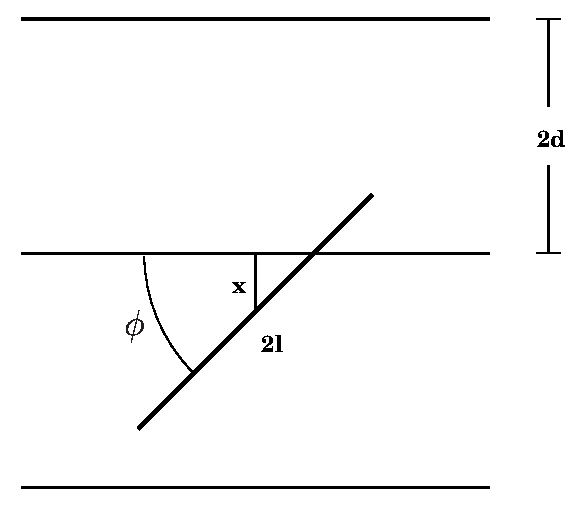
\includegraphics[width=.7\textwidth]{Figures/buffondefinition.eps}
\caption{The Buffon needle problem. Definition of the variables $x$
  and $\phi$.}
\end{figure}

Let us look at the possible positions of the needle in the $x$--$\phi$
plane (see Fig. (\ref{buffonplane})). All positions lying below the
$l\sin \phi$ curve between the abscissa 0 and $\pi$ satisfy the
condition (\ref{buffoncondition}). The surface of this region is
immediately found by integration, $F=2l$. The surface $F$ is a measure
for the set of all positions of the needle which cross one line. On
the other side it is clear that $\pi d$ is am measure for the surface
of all possible ppositions of the half needle. The ratio of the two
measures $ 2l/\pi d$ is the probability we were looking for, i.e.,
\begin{equation}
\label{buffonprobability}
P = \frac{2 l}{\pi d}.
\end{equation}

\begin{figure}
\label{buffonplane}
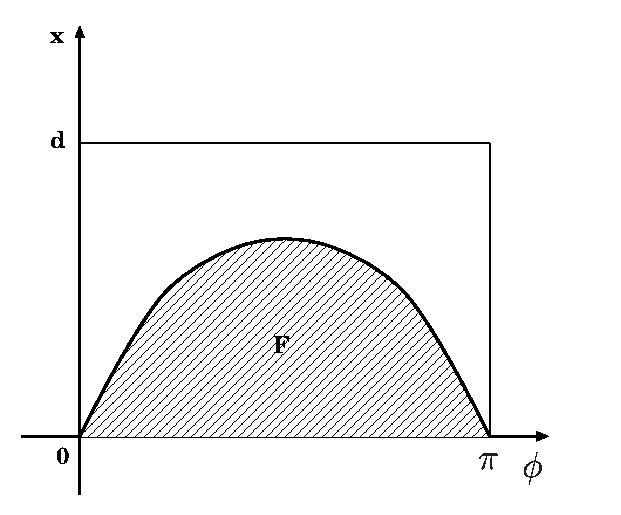
\includegraphics[width=.8\textwidth]{Figures/buffonplane.eps}
\caption{The buffon needle problem. The $x$--$\phi$ plane (schematically).}
\end{figure}

Some years later (??) Laplace 
\footnote{Pierre Simon Marquis de Laplace, $\ast$ Beaumont--en--Auge
  28.3.1749 \dag 5.3.1827 Paris. Laplace was one of the leading french
  mathematicianbs of his time. Before being a member in the Acad\'emie
  des sciences and a Professor at the \'Ecole Normale in Paris (1794)
he was an exmainator at the \'Ecole militaire in Paris, where in 1785
he examined Naplo\'eon Bonaparte. The most important contributions of
Laplace where in celestial mechanics, cosmology, mathematical physics
and, probability theory. In his work ``Th\'eotie analytique des
probabilit\'es'' (1812) he develops  for the first time a systematic
mathematical treatment of probabilistic problems.} recognized that
the idea behind the Buffon needle experiment could be used to evaluate
$\pi$ from the throws of the needles. Today we would call this a
Monte Carlo determination of $\pi$. If we repeat the experiment $N$
times and count the number of times the needle crosses a line $M$, the
probability $P$ can be estimated by the relative frequency of hits
\begin{equation}
\label{buffonestimateP}
P \approx M/N
\end{equation}
and hence we have with Eq. (\ref{buffonprobability})
\begin{equation}
\pi \approx \frac{2lN}{dM}
\end{equation}
Now, let us try to write a Java code for the simulation of the Buffon
needle problem.

\subsection{The Traditional (Procedural) Approach}
The traditional approach is straightforward. You just
draw \verb|N| needles and check each needle if it crosses a
line or not. So there are two subroutine. One creates a new
needle with all four coordinates. And the second one is a 
routine, which just compares the lines with the needle coordinates,
whether it crosses the lines or not. You then count the number
of crossings and you get the final estimate of Pi.
\loadlisting{BuffonProcedural.java}{Listings_Java/BuffonProcedural.java}

First of all we have made use of the \verb|Math.random()| method, which
draws a random number (a double) between 0 and 1. We also used arrays
to store the coordinates and even used arrays as parameters to
subroutines (methods). The remianing of the program should be
selfexplaining.

\subsection{The Object Oriented Approach - Classes and Objects}
\label{sec:Classes_and_Objects}
Before we begin to write the object oriented code 
we have to introduce some formal aspects of the Java language.

\subsubsection{Definition of Objects}
We have already met a lot of object oriented features 
without discussing them in detail.  For example, we already noticed
that the fundamental unit of programming in Java is the {\em class}. A
concise definition of classes and objects in Java could be:
\begin{quote}
A class is a collection of data and methods that operate on that data. In
Fortran or C we call the methods procedures or functions. An object
is an instance of the class, meaning it is a thing to work with. The class
defines the data necessary for the object and the functions which can
operate on them.   
\end{quote}

In other words, like in other languages you can compute only with
primitive types (integer, float, ...) but you can also creat and
manipulate objects. An example already familiar to us, is the  array. 
If you have an array 
object you can call the method \verb|length| to get the number of
elements of the array. 

So what is the difference to the standard function approach here?
Instead of using function arguments you supply the argument by 
putting them in front of the method separated by a point, e.g., 
\verb|args.length|. The missing brackets on the \verb|length| method
is not a misprint, the Java engineers thought it might ease writing
array code, but actually it confuses sometimes. Still it is the
most easy demonstration of calling a method of a class.

To calculate the mean of an array of doubles, you can
either write a method which takes the array as an argument (like you would
in Fortran or C) or you can use the object
oriented feature:

\begin{small}
\begin{minipage}{.47\textwidth}
\textbf{Functions}
\begin{verbatim}
  double[] array = new double[100]; 

  result = mean(array[]); 
\end{verbatim}
\end{minipage}
\begin{minipage}{.47\textwidth}
\textbf{Object Oriented}
\begin{verbatim}
  double[] array = new double[100]; 
  Data dat = new Data(array); 
  result = dat.mean();
\end{verbatim}
\end{minipage}
\end{small}

Look at the third example in this chapter, which demonstrates these two
possibilities in detail.

It is up to you, which version you prefer. But because all programs are
actually classes in Java you have to understand at least the 
most fundamental things about object oriented programming. For a detailed
discussion and introduction, see \cite{javanutshell}.

Just to remind you again, strings are objects and not primitive 
types. To use strings you first have to declare and instantiate a string
object. Here are three possible ways of doing it:
\begin{verbatim}
        String text;
        text = "Test String";
        text = new String();
        text = new String("Test String");
\end{verbatim}
The first line only declares a string object called text and does not
allocate (instantiate) the memory for the value of the object, just
the reference to the value. The second line instantiates and 
defines the String object \verb|text|. The third line instantiates, but
does not define it and the fourth line is like the second line, with
the second line being more efficient in memory consumption and
speed.

\subsubsection{The Code of the Object Oriented Approach}
Now we want to
write a Java code which allows the simulation of the Buffon needle
problem. It is clear that in the problem at hand ``needles'' will play
a central role. Each needle may be described by the $x$-- and
$y$--coordinates of  its two ends. Of course, for each needle we can
check wheteher it crosses a line or not. We draw needles at random so
different needles will have different coordinates. However, needles
have also generic properties which justify to define needles as a class!

The listing of the \verb|Needle| class can be seen below. We are going
to explain basic concepts while discussing this example.
\lstinputlisting{Listings_Java/Needle.java}

\subsubsection{Class variables, Constants and Modifiers}
The needle class has four fields which correspond to the four
coordinates which specify the position of the needle. 
The term fields is used in Java as a synonym for variables.
Furthermore, we
need some specification for the geometry involved in the problem.
Some of the fields  are
defined with the \verb|final| keyword. This is the equivalent to the
const keyword in C. A final field can not be changed anymore.

There is a nice feature to be used with the final keyword. You can
define a final variable, actually computed in an arbitrary method. 
The method is then executed before any other code of the program,
even before the main method. An example would be:
\lstinputlisting[first=12]{Listings_Java/TestFinal.java}
 
The variable \verb|cross| is declared to be \verb|static|.  This
modifier 
defines a field (variable), which is belonging
to the class and not to the object. So every object of that class 
has the same value for a \verb|static| field. The \verb|public| modifier
on the other hand defines a field or method, which is special to 
an object not to the class -- this is also called an instance field or
method, the \verb|static| version is called a class variable or
method.

In Table \ref{tab:modifiers} we give an overview of some available modifiers.
\begin{table}[htbp]
  \begin{center}
    \leavevmode
    \begin{tabular}{l|p{8cm}}
     Modifiers &                                 \\ \hline \hline
     final & variables may not be changed, methods can not be overwritten,
             classes may not be subclassed\\\hline
     public & accessible from anywhere\\ \hline
     static & defines a top-level class, a class variable (field) or 
                 a class method\\\hline
     private & only within the defining class visible, not in other 
               packages, even if subclass of this class\\\hline
     protected & accessible within the package in which it is defined and
                 within subclasses\\\hline
     (none) & accessible only in its package\\
    \end{tabular}
    \caption{Overview of some available modifiers in Java. For a complete
      overview take a look at page 230-234 in \cite{javanutshell}.}
    \label{tab:modifiers}
  \end{center}
\end{table}
A graphical representation of the access control of variables and
objects is in figure \ref{fig:ModifiersGraphics}.
\begin{figure}[htbp]
  \begin{center}
    \includegraphics[width=.7\textwidth]{Figures/ModifiersGraphics.eps}
    \caption{A graphical overview of the access control of variables and objects/classes in Java.}
    \label{fig:ModifiersGraphics}
  \end{center}
\end{figure}

It is important to remark that
class variables and methods are the closest relatives to global 
variables in all the other languages. They are accessible from all
classes, but still are belonging to a class. So you could have two
class methods with the same name, but for different classes.

Having fixed also some constants, e.g. $\pi$ and the distance between
parallel lines, we have to initialize the class. This is done by means
of the constructor.

\subsubsection{The constructor}
An important part of any class is the constructor of the class. This is
the method (function), which is called when an object of this
class is instantiated. It always has the same name as the class itself.
The constructor can have zero or more arguments and you can even
have different constructors depending on the parameters provided by
the calling syntax.

The constructor of a class ALWAYS calls the constructor of its
superclass, so it is good practice to write \verb|super();| at the
beginning of a constructor to indicate this feature. Because the 
construtor of the super class also calls the constructor of its super
class again, this is called ``Constructor Chaining''.

In our example a needle is initialized in the following way. We draw
at random the four coordinates \verb|needleX1|, \verb|needleX2|,
\verb|needleY1|, and \verb|needleY2| which determine the position of
the first needle. Note, that we have made use of the keyword
\verb|this|.
This keyword is always required when the argument of a method
or a local variable in a method have the same name as one of the fields
in the class. If the method is simple, as it is the case here, it is
not necessary to be that careful.

Here in our example, the constructor just sets the four coordinates
and does not need any parameters to instantiate the needle.

\subsubsection{Class methods}
Having initialized the class we now want to define some methods in our
\verb|Needle| class. There is only one method in our class, which
is the \verb|crossinspection()| method.
The return type of methods always has to be specified, if
there is no return value you have to use the \verb|void| statement
(as in C). The value to be returned is specified by the return keyword.

The method \verb|crossInspection| checks whether
a needle crosses a line or not. The \verb|crossInspection| method
returns a boolean telling you, if the needle crosses a line or not.
Note that the variable \verb|cross| has
been defined as a class variable with the help of the modifier \verb|static|
and gets incremented every time you check a needle, which crosses a line.
With this method our \verb|Needle| class is complete.

Next we need to look at the class \verb|Buffon.java| which contains the
\verb|main| method and demonstrates how to use the \verb|Needle| class.
\loadlisting{Buffon.java}{Listings_Java/Buffon.java}

By defining the \verb|Needle| class in Java, we have created a new
data type. Variables of this type can be declared by
\begin{verbatim}
Needle draw;
\end{verbatim}
\verb|draw| is simply a name that refers to a \verb|Needle|
object (references the object). 
Creating dynamically an object
is done with the help of the \verb|new| keyword
\begin{verbatim}
draw = new Needle();
\end{verbatim}
Next, in a \verb|for| loop we draw \verb|N|  needles and with the help
of the \verb|crossInspection| method we check whether the needles
cross the lines or not and the class variable \verb|cross| is set
accordingly. Finally, the result, i.e. the estimated value
for $\pi$ is printed.


%%%%%%%%%%%%%%%%%%%%%%%%%%%%%%%%%%%%%
\subsection{A Random Number Generator}
Since the concepts we just introduced are quite abstract it may be
useful to see them in action with the help of a second example.
So let us write a class, which calculates random numbers uniformly
distributed bewtween 0 and 1. To this end we write a class
\verb|RandomNumber|. It has three fields (variables), two of them are
defined with the \verb|final| keyword.
\loadlisting{RandomNumber.java}{Listings_Java/RandomNumber.java}
In our example, we just set the seed in the constructor and as 
you can see you have to supply the seed, when you instantiate the
generator. Most of the constructors don't even need a parameter to 
instantiate the object. 

Then the method \verb|nextRand()| is defined and returns the next
random number calculated using a congruential method\footnote{See later 
in this book for details about how to generate random numbers.}. 

Now we have to write a program (class), which uses this class to 
calculate the average of some random numbers.
\lstinputlisting{Listings_Java/UseRandomNumber.java}
The class is called \verb|UseRandomNumber| and just contains the
main method. First we instantiate (create) an object of class
\verb|RandomNumber|. Then we create an array and in a loop we
create \verb|N| random numbers using the \verb|nextRand()| method
of our class applied to the object we just created. The remaining
part has already been explained.

Remember that we have to put both programs in one directory called
\verb|simu|, because we have used the \verb|package| command. Here it
was just to get you acquainted with these terms.

%%%%%%%%%%%%%%%%%%%%%%%%%%%%
\subsection{Calculating Moments}
A third example demonstrates how to create a class for calculating
some statistical measures for data sets. Here we show the
different approaches of programming models in Java. 
You have basically three choices:
\begin{enumerate}
\item You can use the ``program in one file'' approach: 
\lstinputlisting{Listings_Java/Moments_all.java}
\item You can use the ``traditional procedural'' approach:
\lstinputlisting[first=23,last=28]{Listings_Java/Moments_procedural.java}
\lstinputlisting[first=35,last=42]{Listings_Java/Moments_procedural.java}
\item You can use an object oriented approach, the first class is always
  the main program using our own class and the second one is the
  code for the data class itself:
  \begin{enumerate}
  \item Use an empty constructor: 
    \lstinputlisting[first=23,last=28]{Listings_Java/Moments_object.java}
    \lstinputlisting{Listings_Java/MomentsData.java}
  \item Use of a constructor:
    \lstinputlisting[first=25,last=33]{Listings_Java/Moments_object2.java}
    \lstinputlisting{Listings_Java/MomentsData2.java}
  \end{enumerate}
\end{enumerate}

%%%%%%%%%%%%%%%%%
\subsection{Interfaces and Abstract Classes}
Abstract classes/methods 
are also special classes, which can not be instantiated
and contain no code for the (abstract) methods. If you define
some methods, which contain no code as abstract, you have to 
define the whole class as abstract. You can subclass from an 
abstract class and override the abstract methods. You do not have
to override all abstract methods, but then the subclass is abstract
too.

An even more important concept in Java is the interface.
An interface is basically a(n abstract) class, which does not implement 
all the
methods defined in the class. All methods have automatically the public
modifier and are abstract.
Therefore you can create classes defining abstract methods,
which should be implemented (maybe system dependent, e.g. if you use
the native modifier) somewhere else. Interfaces can be subclassed
to create new interfaces.

Most of the GUI classes of the AWT introduced later are
actually interfaces or abstract classes and not just ordinary classes.
Very useful is this concept for passing methods as arguments to
other methods (see section \ref{sec:PassingArguments}).


%%%%%%%%%%%%%%%%%%
\subsection{Extending (Inheritance) and Overloading (Overriding) Classes}
Often you want to define subclasses, which should inherit all
the methods and fields from another class. This is easily done
in Java by extending a given class. The meaning of subclassing is the
notion of data hiding or encapsulation. For example you can write
a subclass, which can not access all the variables of the super class,
therefore hiding some details. 

You can reference the super (parent) class by applying the
\verb|super| modifier in front of a method or variable of
the parent class. And the \verb|this| modifier always refers to
the actual class. 

You can also have equal names for a variable in the super class and the
child class, which means you have to reference the variables explicitly
by using the \verb|super| or \verb|this| keywords. If you want to refer
to a variabel two classes up from the actual class, you have to use
the notion of ``shadowing'' \cite[]{javanutshell}, which is a kind of
casting with classes. 

If you define a class to be final, it can not be extended.
For example the java.lang.System class is a final class.

Different from C++,  you can not inherit from more than one class
in Java, meaning that there is always only one superclass for each
class. 
The only way of having multiple inheritance is by using
interfaces, which we will not cover extensivly in our introduction.

If you write a subclass you can overwrite methods already defined
in the super class. This is called overloading of methods,
analogous to the C++ overloading. But in C++ you can even
overload operators like +, -, etc., which is not possible (in Java 1.1) yet.

A simple example is given by the
HelloWorld\_Applet.java program in section \ref{sec:Applet}.
There we have extended the Applet class of the Java.applet package
and therefore making our program a subclass of the Applet class.
So we inherited all the methods and fields of that class. Then we
overloaded the \verb|paint()| method to display our message. 
In the words of object oriented programming, writing an applet is
called: defining a subclass of the Applet class and overloading
the methods of the Applet class as necessary.

One nice and important feature in Java is, that all classes which
do not have an explicit parent, inherit from the \verb|java.lang.Object| 
class. So you can call this class the father of all classes.
There are only a few methods defined in this (abstract) class,
which you can always override. For example the \verb|toString()| 
method is in \verb|java.lang.Object|. If you override this method,
you can define your own objects, which can then be printed by
the usual \verb|println()| commands. In table \ref{tab:JavaLangObject}
all methods defined in \verb|java.lang.Object| are displayed.
\begin{table}[htbp]
  \begin{center}
\begin{small}
\begin{verbatim}
public boolean equals (Object obj);
protected Object clone() throws 
               CloneNotSupportedException, OutOfMemoryError;
public String toString ();
public int hashCode(); 
protected void finalize() throws Throwable;
\end{verbatim}
\end{small}
    \caption{All methods belonging to the (abstract) 
               \texttt{java.lang.Object} class.}
    \label{tab:JavaLangObject}
  \end{center}
\end{table}

%%%%%%%%%%%%%%%%%%%%%%%%%%%%%%%%%%%%%%%
\subsection{The System Class: Screen-Output and Keyboard-Input}

Now we are in a place to discuss the \verb|System.out.println()| statement
already used in the ``HelloWorld'' program. This is calling the
\verb|println()| method of the \verb|PrintStream| class of the java.io 
package. And the \verb|out| is a variable from the System 
class of the java.lang package, referencing the \verb|PrintStream| class. 

There are also two more variables called \verb|err| and
\verb|in| for error output and data input. 
The java.lang.System class in general provides an platform-independent 
interface to some system functions.

Here an example, which demonstrates a few things already learned and
explains how to get input from the keyboard:
\inputlisting{Listings_Java/System_Class.java}
It waits for an user input and just echoes the typed characters
until you type the word ``Java''. Let us analyze the program:

First look at line 19, where we have used the \verb|print()| method
of the System class. It does the same as \verb|println()|, but does not
jump to the next line after the output.

Then take a look at line 23, where we compare two strings. As you see
you have to use the \verb|equals()| method of the String class to
compare the value of two strings and not the references. 
In line 25 we use the string concatenation operator $+$ for the output.

By the way, you have probably already noticed, that 
the \verb|for(;;)| loop in line 17 is a endless loop.

The actual input takes place in line 21, where we assign the input
to the string \verb|line|. The method used is \verb|readLine()|, which
is a method of the \verb|BufferedReader| class. It reads input until
a carriage return is reached. The actual object of the 
\verb|BufferedReader| class is created in line 13. To that end we have
to create a Reader class for the \verb|InputStream| called \verb|in|
just mentioned above (this is done in line 11).

Because we are using I/O commands, we have to take care of exceptions
which can occur during the I/O. For that reason we have to use the
\verb|throws IOException| statement in the definition of the main
class (see line 7).

A last remark concerns the escape codes used in line 15 and line 25.
The first one, $/$'' displays a quotation mark and the second
one a newline.
To include arbitrary formatting (escape) characters
to the string supplied to the print() and println() methods, you
can use similar to C the \verb|\n|, \verb|\t| or \verb|\\| codes
to get a newline, a tab or a backslash in the output. You should 
also note that, if you use e.g. \verb|System.out.println(5+7)| you
get \verb|12| as output, so if you want to see \verb|5 7| you have
to use \verb|System.out.print(5+" "+7)|.

Although this looks very complicated, if you don't want to go into
details, just copy this part to your own program and your are done.
But after you got used to object oriented programming you won't have
any problems understanding the code above anymore.

\subsubsection{Easy Input and Lava Rocks printf()}
\label{sec:LavaRocks}
Another easy solution is to use the \verb|EasyIn| and the
\verb|Printf()| methods, supplied by our \verb|simulation| class
and the ''Lava Rocks''\footnote{This is a freely available package,
containing some easy to use methods, mostly for C programmers
who switched to Java. For details see \cite{LavaRocks}.} package.

\paragraph{Easy Input}
You can easily use these methods to get input from keyboard
for different primitive data types. For example to input
a primitive data types, you just use
\begin{small}
\begin{verbatim}
import simulation.*;
 .....
 double  d = EasyIn.readDouble();    // reads double from System.in
 int     i = EasyIn.readInt();       // reads int from System.in
 float   f = EasyIn.readFloat();     // reads float from System.in
 boolean b = EasyIn.readBoolean();   // reads boolean from System.in
 .....
\end{verbatim}
\end{small}

\paragraph{Lava Rocks -- printf()/sprintf()/fprintf()}
To use the Lava Rocks package you could write a code like
\begin{small}
\begin{verbatim}
 import lava.clib.*;
 .....
 int i=100;
 float f=165.234f;
 Stdio.printf ( "%8d and %8.1f : test text\n", new Object [] { 
                             new Integer(i), new Float (f) } );
 .....                 
\end{verbatim}
\end{small}
Remember that you need the \verb|lava.jar| file in the classpath.
The output will look like
\begin{verbatim}
     100 and    165.2 : test text
\end{verbatim}
If you are familiar with the C routines, then you can find all
the modifiers used for formatting the different types of variables
in table \ref{tab:PrintfModifiers}.
\begin{table}[htbp]
  \begin{center}
    \begin{tabular}{cl}
      Modifier & Type to be formatted \\ \hline
      \%bd & byte \\
      \%hd & short \\
      \%d & signed integer \\
      \%ld & long \\
      \%u & unsigned integer \\
      \%o & unsigned octal integer \\
      \%x / \%X & unsigned hexadecimal integer (lower or uppercase)\\
      \%f & float \\
      \%lf & double \\
      \%e / \%E & float, scientific notation \\
      \%g / \%G & float, same as f or e, depending on value \\
      \%s & String \\
      \%c & character\\
      \%p & object identity hash code in unsigned hexadecimal \\
      \%$\backslash$n & platform independent line seprarator\\
      \%n & counts characters\\
    \end{tabular}
    \caption{All possible modifiers to be used in the format 
      string given to the printf()/sprintf()/fprintf() methods supplied 
      by the Lava Rocks package.}
    \label{tab:PrintfModifiers}
  \end{center}
\end{table}
The modifiers represent the place, where the actual value of the variable 
has to be inserted before the output is sent to the screen (or file, 
or string). So you have to make sure that the order of the modifiers and
the order of the supplied variables is correct, otherwise you get
unpleasant results or strange errors.

There are three additional things to mention: 
If you use the
same format string (the first argument to the printf method) 
very often, you can speed things up by saving the format string
and only use the variable every time, like:
\begin{small}
\begin{verbatim}
   import lava.clib.stdio.*;
   .....
   PrintfFormatString fmt = 
      new PrintfFormatString ("%8d and %8.1f : test text\n");
\end{verbatim}
\end{small}
Now you can use \verb|fmt| instead of the string in all printf commands
and it will be much faster.

There is also an ''easier'' way of using printf without creating
an object array, which is much more inefficient and should be avoided.

And there is a platform neutral code for newlines: Use \verb|%\n| instead
of \verb|\n| in the format strings and you always get a newline,
no matter which platform you run the program.

The same holds for the other two methods \verb|sprintf()|, which writes
the formatted output to a stringbuffer (we will discuss this in section
\ref{sec:FileIO} and in section \ref{sec:Symphony} in more detail.),
and \verb|fprintf()|, which writes the output to a file (actually a
Writer, see section \ref{sec:FileIO}).

There is another free implementation of the printf command for
Java called \verb|Format.java| of the \verb|corejava| package.
But it has much less functionality and so we decided to use
the Lava Rocks implementation.

%%%%%%%%%%%%%%%%%%%%%%%%%%%%%%%%%%%%%%%%%%%%%%%%%%%
\subsection{Passing Arguments to Methods}
\label{sec:PassingArguments}
We want to review all the aspects concerning the passing of
arguments to methods or -- for former FORTRAN programmers --
passing arguments to subroutines/functions.

\paragraph{Global Variables}
First of all there is of course always the possibility to 
pass variables as global variables. This is easy to use,
but it makes it difficult to follow a program structure.
So it is preferred to use arguments to methods in an
argument list.

\paragraph{Primitive Data Types}
The important point to note here is that Java always
passes primitive data types by value and all the other
arguments by reference (reference data types). 
This means that all primitive
variables of the argument list can be changed within
the method and the dummy variables used in the method 
can be viewed as local variabels.

\paragraph{Reference Data Types}
But the reference data types (e.g. arrays, objects, etc.)
are passed by reference and therefore only the memory
address is passed to the method. That is again the reason that
by using the standard assignment or comparison operators,
you do not compare the values of the reference data type, but
the memory addresses where the data is stored. Therefore there
is the \verb|equals()| operator used for comparing reference data
types. By the way there is no method
of getting the actual memory address for a reference data type,
which would be a severe security problem.

If you pass a reference data type to a method it should be
clear, that every change of the dummy variable used for
the reference data type used in the method, will result in a change
of the passed reference variable. So for example for arrays:
\begin{lstlisting}{}
  .....
  public void main (String[] args) {
    ...
    int[] array = {1,2,3,4,5};
    test(array);
    ...
  }
  public void test(int[] dummyarray) {
    int length=dummyarray.length;
    for (int j=0; j<length; j++) {
      array[j]=0;
    }
  }
  .....
\end{lstlisting}
In this example we pass an array of integers, where the values are all 
not zero. In the subroutine we change the values of the dummyarray.
But we passed only the memeory location, so the change is actually
a change in the \verb|array| array. If you print the result after
the call to the method, all elements are zero!

If you now think about changing a primitive data type inside a method 
passed it, there is no simple way of using reference types for 
them. 

\paragraph{Instance Variables}
A nice and clear way of passing arguments between methods, is
using instance variables. The problem here is that you have
to create a new class and define instance variables for it.
Then you can instantiate an object of this new class and
change the values of the instance variables from the main
program or the methods therein. But still you have the problem
of passing the instance to the methods.

\paragraph{Methods (Functions) as Arguments} 
Especially for scientists it is of great importance to know how
to pass a function (method) to another method.

The first solution would be to write a method as a class method,
therefore accessible from every instance of the class and
so you do not need to pass the method as an argument at all.

The second solution is much more versatile and general.
But as always you have to do more work. You need an interface,
which defines the function you would like to pass to a method
(Declaration). Then you need a class, which implements this
interface, therefore representing the real function (Implementation).
And at last you write your program/class, which instantiates
the former class and now you can pass the function by reference
to all methods you like (Usage).  

Here a short example:
\paragraph{Declaration} 
\begin{verbatim}
  interface function {
    double f (double x); 
  }
\end{verbatim}

\paragraph{Implementation}
\begin{verbatim}
  class SquareFunc implements function {
    public double f (double x) {
       return (x*x) ;    //  <----- here is the actual function
    }
  }
\end{verbatim}

\paragraph{Usage}
\loadlisting{TestPassingFunctions.java}{Listings_Java/TestPassingFunctions.java}

%%%%%%%%%%%%%%%%%%%%%%%%%%%%%%%%
\section{Structure and Overview of Java}

%%%%%%%%%%%%%%%%%%%%%%%%%%%%%%%%%%%%%%%
\subsection{Keywords and APIs in Java 1.1 and Java 2}

Here we list all the standard packages (APIs) included in the Java 1.1
language standard. The important packages (for our purposes) are
written in small caps.

\paragraph{Java 1.1 packages}
\begin{description}
\item[\textsc{java.applet}] includes the superclass of all Java applets (small package)
\item[\textsc{java.awt}] the Abstract Windowing Toolkit (large package)
\item[java.awt.datatransfer] provides data exchange between programs
\item[\textsc{java.awt.event}] event handling for the AWT (Mouse, etc.)
\item[java.awt.image] rarely used classes for image processing (use AWT) 
\item[java.awt.peer] rarely used interfaces for the AWT
\item[java.beans] interfaces and classes for beans programmer
\item[\textsc{java.io}] all the input/output classes (very big)
\item[\textsc{java.lang}]  central Java language classes (largest package)
\item[java.lang.reflect] part of the Java Reflection API (small)
\item[\textsc{java.math}] arbitrary precision arithmetic (small)
\item[java.net] networking package
\item[java.rmi] RMI is Remote Method Invocation. It is a mechanism that enables an object on one Java virtual machine to invoke methods on an object in another Java virtual machine. 
\item[java.rmi.dgc] RMI distributed garbage-collection (DGC). 
\item[java.rmi.registry] Methods to access the RMI registry.
\item[java.rmi.server] RMI server classes and methods.
\item[java.security] A security framework. This includes classes that implement an easily configurable, fine-grained access control security architecture.
\item[java.security.acl / java.security.cert / java.security.interfaces / java.security.spec] Additional security features.
\item[java.sql] Provides the JDBC (Java Database Connectivity) package. JDBC is a standard API for executing SQL statements.
\item[java.text] for writing internationalized programs (date, time, etc.)
\item[\textsc{java.util}] useful classes, often used, e.g. millisecond time,
  calendar, random numbers, vectors, etc.
\item[java.util.zip] data compression and decompression classes
\end{description}

\paragraph{Java 2 packages}
Additional API packages in Java 2 are:
\begin{description}
\item[java.awt.color] Provides classes for color spaces.
\item[java.awt.dnd] Provides interfaces and classes for supporting drag-and-drop operations.
\item[java.awt.font] Provides classes and interface relating to fonts. It contains support for representing Type 1, Type 1 Multiple Master fonts,
OpenType fonts, and TrueType fonts. 
\item[java.awt.geom] The Java 2D classes for defining and performing operations on objects related to two-dimensional geometry. 
\item[java.awt.im] Classes and an interface for the input method framework. This framework enables all text editing components to receive Japanese, Chinese, or Korean text input through input methods. 
\item[java.awt.image.renderable] Classes and interfaces for producing rendering-independent images.
\item[\textsc{java.awt.print}] A general printing API, including document types, 
  page setup and formats and job control dialogs.
\item[java.beancontext] A bean context is a container for beans and defines the execution environment for the beans it contains.
\item[java.lang.ref] Provides reference-object classes, which support a limited degree of interaction with the garbage collector.
\item[java.rmi.activation] Provides support for RMI Object Activation.
\item[java.util.jar] For reading and writing the JAR (Java ARchive) file format, which is based on the standard ZIP file format with an optional manifest file. 
\item[javax.accessibility] Defines a contract between user-interface components and an assistive technology that provides access to those components. 
\item[\textsc{javax.swing}] Provides a set of "lightweight" (all-Java language) components that, to the maximum degree possible, work the same on all
platforms. 
\item[java.swingx.*] There are 15 more packages in the Swing package, which we are not describing here in detail. Take a look at the Swing tutorial or documentation.
\item[org.omg.COBRA] Provides the mapping of the OMG CORBA APIs to the JavaTM programming language, including the class ORB, which is implemented so that a programmer can use it as a fully-functional Object Request Broker (ORB).
\item[org.omg.*] 6 more packages are provided for using COBRA with Java. See the API documentation.
\end{description}

\subsubsection{Reserved words in Java}
The following words are reserved for Java and can not be used for names
of classes, variables or methods:
\begin{verbatim}
abstract, boolean, break, byte, byvalue, case, cast, catch, char,
class, const, continue, default, do, double, else, extends,
false, final, finally, float, for, future, generic, goto, if,
implements, import, inner, instanceof, int, interface, long,
native, new, null, operator, oouter, package, private, protected, 
public, rest, return, short, static, strictfp, super, switch, 
synchronized, this, throw, throws, transient, true, try, var,
void, volatile, while, widefp
\end{verbatim}

%%%%%%

\subsection{Name Conventions in Java}
In order to make the Java codes more readable it is customary to stick
to the followinh nam conventions.

\paragraph{Classes and Interfaces.} The names of classes and interfaces
  should consist of one or more words which are joponed together. They
  should describe appropriately the class and the interface. 
The first lette of the name is an uppercas letter. If the
  class name consists of more then one word each word after the first
  one begins with an uppercase letter, e.g., \verb|Needle|,
  \verb|Reader|, \verb|StringToken|.

\paragraph{Methods.} The names of methods are verbs or verb--phrases. 
  They begin with lowercase letters. If the name consists of
  more than one word, the second and all the following words begin
  with an uppercase letter. To give some examples:
\begin{itemize}
\item methods, which set the value of a variable or return the value of
  a variable begin with \verb|set| or \verb|get|; e.g.,
  \verb|setName|, \verb|getData|.
\item methods, which check some condition and return a result  get the
  prefix \verb|is|, e.g., \verb|isSmaller|.
\item methods, which simply perform some conversions are characteized
  by the returned type and have the prefix \verb|to|, e.g.,
  \verb|toString|.
\end{itemize}

\paragraph{Instance Variables.} Names for instance variables are
  words, nominal phrases, or short--hand notations. Like names for
  methods the word begins with a lowercase letter and all following
  words begin with an uppercase letter, e.g., \verb|next|,
  \verb|dataVector|,
\verb|minValue|.

\paragraph{Local variables or parameters.} Local variables should get
  short  names. Usually, they are named ny sequences of small
  letters. Typical examples are acronyms (the first letter of each
  word) of the name of the class for a variable, which keeps a
  reference to an instanace of the class, e.g., \verb|v| for Random
  Variable or short--hand notations, e.g., \verb|minx| for the minimal
  value of the variable x. Single letter names should be avoided,
  unless for temporary variables or variabl"oes which are used in
  loops or for variables with an uncertain value of some type:
\verb|b| for \verb|byte|, \verb|c| for \verb|char|, \verb|d| for
  \verb|double|, \verb|e| for Exception, \verb|f| for \verb|float|,
  \verb|i|,
\verb|j|, \verb|k| for \verb|int|, \verb|l| for \verb|long|, \verb|o|
  for \verb|Object|, \verb|s| for \verb|String|.

\paragraph{Constants.} The names of constants may be composed by one
  or more words. All characteres are upper--case letters and the words
  are joined by \verb|_|, e.g., \verb|PI|,  \verb|MIN_VALUE|.

\paragraph{Packages.} Packages, which are only used locally are
  identified by a name which begins with a lower--case letter. This
  word can not be \verb|java|; this keyword is reserved for
  standard Java classes.



\subsection{Java Documentation}
As the time of writing the JDK (1.1 or 2) is distributed in
two parts. The first one is the software itself, including all
the tools and programs necessary to write Java programs. 
The second one is the API documentation. 
In the directory \verb|JAVA_HOME|, on UNIX this could be 
\verb|/usr/local/jdk1.2|, \verb|/usr/local/lib/jdk1.2| or 
\verb|/usr/lib/jdk1.2| and on Windows this might be \verb|c:\jdk1.2|, 
you can find all the documentation in the subdirectory
\verb|docs|. It is of course best viewed using a web browser
starting with the page \verb|jdk1.2/docs/index.html| 
(see also figure \ref{fig:JDKFiles}).
\begin{figure}[htbp]
  \begin{center}
    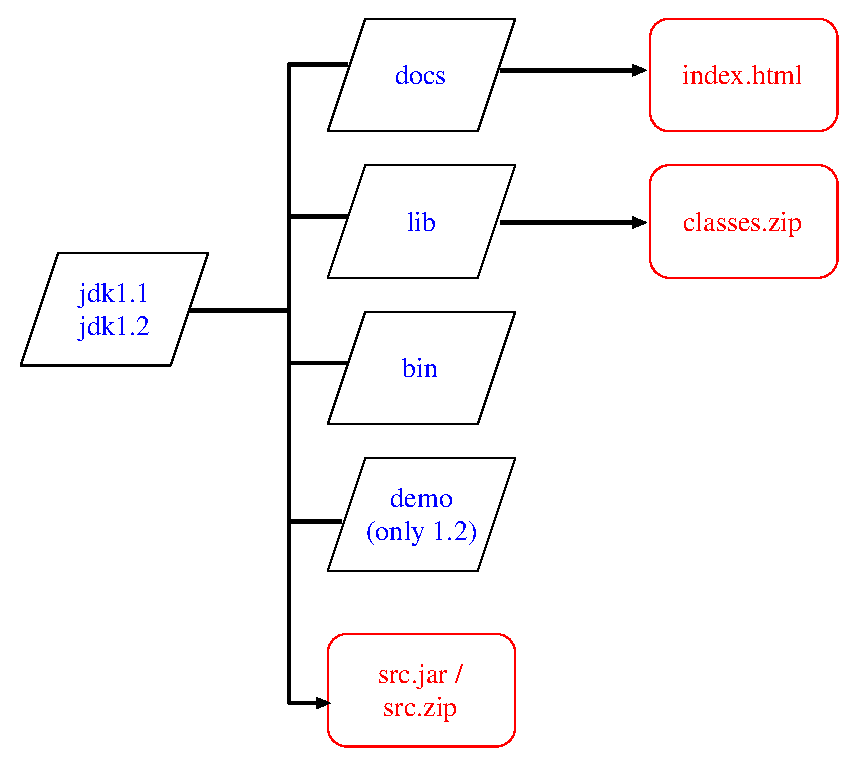
\includegraphics[width=.6\textwidth]{Figures/JDKDocumentation.eps}
    \caption{The file structure of the JDK distribution, both the binary and the documentation package.}
    \label{fig:JDKDocumentation}
  \end{center}
\end{figure}


%%%%%%%%%%%%%%%%%%%%%%%%%%%%%%%%%%%%%%%%%%%%%%%%%%%%%%%%%%%%%%%%%
\section{Applications and Applets Revisited}

After learning many things about object oriented programming,
we want to recapitulate the basic differences and features of
the two possible ways of writing and starting Java programs.

\subsection{Application}
A Java application is in the traditional language a ``normal'' program.
In Java slang it is a class, which only has to have a \verb|main|
method, which has to be \verb|static| and \verb|public|. This is also of course the
entrance point, if you start the Java application. Then the program
executes sequentially the code given in the main method (of course it
goes parallel, if you use threads somewhere in the application - see
\ref{sec:ParallelJava}). There are no restrictions of any sort using
features in an application.


\subsection{Applet}
An applet is a Java class, which can be loaded into a virtual machine
and can then be executed their. For example a web browser could load
the applet, check if it is an applet allowed to be started on the
machine the browser is running on and then ``starts the applet''.

This is basically the most confusing part of an applet: What are the
instructions, which get executed when the browser ``starts the applet''?
To that purpose go ahead and write a simple program 
(see e.g. \verb|ShowTrace.java|), which only 
prints out the place where the execution just takes place and ``start''
the Java class on the command line as an application, in the appletviewer
as an applet and in a browser as an applet. What you will get is shown
in figure \ref{fig:LineOfExecution}.
\begin{figure}[htbp]
  \begin{center}
    \leavevmode
    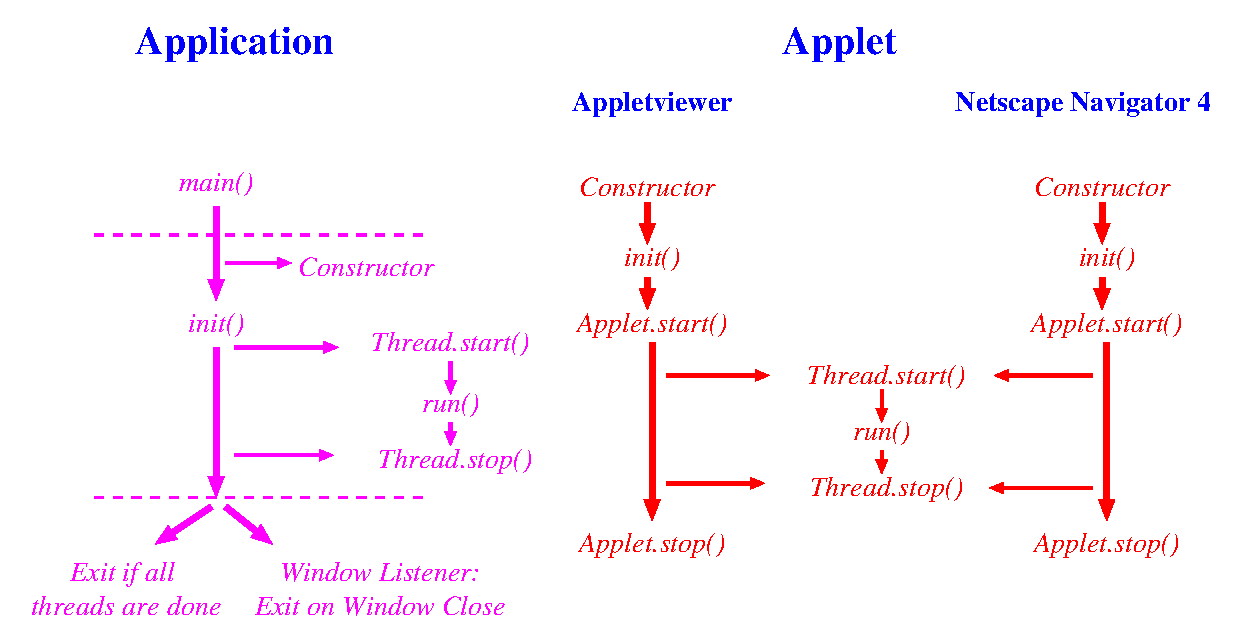
\includegraphics[width=\textwidth]{Figures/LineOfExecution.eps}
    \caption{The line of execution in an application and an applet in
        the appletviewer or the Netscape Navigator V4.08. For the application
        only the part above the first line and below the second line are
        actually the parts, which can not be avoided. The remaining
        part is just provided to show you how to write an application,
        which can be used as an applet, too.}
    \label{fig:LineOfExecution}
  \end{center}
\end{figure}

So for the applets you have to write (implement) at least the 
\verb|init()| method to get things going. But now you will ask, why did we
not supply an  \verb|init()| method when we wrote our first 
HelloWorld applet? The answer is we did, but we did not write it explicitly,
because we left it empty. The trick was that for an applet there is
always another thread (see \ref{sec:ParallelJava} for an introduction to threads)
running, which takes care of (re)painting the windows (panels) used by the applet.
This thread is a method of the AWT package (see \ref{sec:AWTIntro}) and
the method is the \verb|paint()| method. And in the    HelloWorld applet
we have overriden the \verb|paint()| method to display our message.

Actually the threads and methods used for painting and repainting
the windows or panels is a little bit more tricky and involved, so we
have to postpone the discussion to a later chapter. Here only the basics:
There is a method \verb|repaint()|, which calls the \verb|update()|
method and that in turn calls the \verb|paint()| method, when there is time
to do so. This sounds very complicated in the first place, but 
it will be resolved later on.

There is another issue to be addressed here in the context of applets.
So far we have always written a seperate HTML file to use with the
appletviewer, which then in turn calls the applet itself. The burden
of having two files for one applet can be avoided by putting the
HTML Code at the beginning of the Java class file in a comment. Then
if you call the appletviewer with the Java class file 
it executes the HTML code supplied
in the Java class file and starts the applet. It even starts in
the Netscape Navigator, although it probably makes no sense for
large programs embedded in a set of HTML pages kept uptodate in a
different way as the Java source code. But it certainly eases
writing small applets and getting not confused by too many files on
your disks. 

Here a small example showing the described feature:
\inputlisting{Listings_Java/test_Applet.java}
You can start it (first you have to compile it) 
by typing \verb|appletviewer test_applet.java| or 
in the Netscape Navigator type 
\verb|file:/home/user/test_Applet.java|\footnote{You have to substitue the path 
  by an appropiate one for your system and configuration.}.
Then on the command line or the terminal with which you started the browser  
you see the short message.


\subsection{Programs as Applets and Applications}
To write a class to be run as an applet and an application
you can use figure \ref{fig:LineOfExecution} to get the correct order
of the methods, which get called in either case. As an example, we have used
in later chapters for the bigger programs the following philosophy
to have the programs runs as applet as well as a standalone application:
\inputlisting{Listings_Java/TestAppletApplication.java}


%%%%%%%%%%%%%%%%%%%%%%%%%%%%%%%%%%%%%%%%%%%%%%%%%%%%%%
\section{Higher Mathematics in Java}

\subsection{Standard Mathematical Functions in Java}
\label{sec:Standard_Math}

The standard mathematical functions of Java are declared in the 
java.lang.Math class, which consists of static constants and methods
for common mathematical manipulations. 
It contains sine, cosine, logarithm, exponential,
square root and much more. Do not confuse this class with the
java.Math class, which was introduced to Java 1.1 for arbitrary
precision arithmetic -- we are not discussing this, read the
API documentation for details.

Java math is always conforming to the IEEE 754 standard and all
algorithms used in the math API are guaranteed to produce the
same results as those from netlib's 
\emph{Freely Distributable Math Library}\footnote{Called \texttt{fdlibm}.
Netlib is a collection of mathematical software, papers and databases.
It is located at the ORNL (Oak Ridge National Lab in Tennessee) and UTK (University
of Tennessee at Knoxville), but there are many other mirror sites.
Fdlibm is available online from 
\href{http://www.netlib.org/}{http://www.netlib.org/} or
\href{http://www.hensa.ac.uk/ftp/mirrors/netlib/}%
           {http://www.hensa.ac.uk/ftp/mirrors/netlib/}}.
\verb|fdlibm| is a C library for machines supporting the IEEE 754 floating
point artihmetic initially developed by SUN.

Some useful constant in the \verb|Math| class  are \verb|Math.Pi|
($\pi$) and \verb|Math.E| ($e$).



In the following table we have summarized some of the most useful the 
\verb|Math|. Note, that all angles are in radins and allparameters and
return values are double (unless otherwise stated). 
Here is a table of the methods:
\begin{table}[htbp]
\caption{Some useful mathenatical fuinctions defined in the
  java.lang.Math class.}
  \begin{center}
    \leavevmode
    \begin{tabular}{ll}
      abs(x) & absolute value \\
      acos(x)/asin(x)/atan(x) & arcus cosine/sine/tangent \\
      atan2(x,y) & arctangent (x/y)  \\
      sin(x)/cos(x)/tan(x) & sine/cosine/tangent\\
      exp(x) / log(x) & exponential and natural logarithm \\
      ceil(x) & smallest whole number $\ge x$ \\
      floor(x) & largest whole number $\le x$ \\
      rint(x) & x rounded to the nearest integer; \\
             &  if neither integer is
                        nearer, rounds to the even one. \\
      round(x) & (int) floor (x+0.5) for float x \\
       ~       & (long) floor(x+0.5) for double x \\
      pow(x,y ) & $y^x$\\
      min(x,y)/max(x,y)  & minimum (maximum)  of x and y for any numeric type  \\
      sqrt(x) & square root of a double x\\
      random() & random numbers (use java.util.Random class)\\
      IEEEremainder(x) & special remainder function \\\hline
      & \textbf{New in Java 2:} \\
      toRadians(angle) & converts degrees to radians\\
      toDegrees(rad) & converts radians to degrees \
    \end{tabular}
    \caption{Overview of the mathematical methods available in Java 1.1 in the java.lang.Math class.}
    \label{tab:math_table}
  \end{center}
\end{table}

These are all class methods, so they can be called from anywhere.
Here are some examples:
\begin{verbatim}
 a=Math.exp(2.1);        // e to the 2.1
 distance = Math.sqrt(Math.pow(x,2)+Math.pow(y,2));  // Euclidean distance
\end{verbatim} 
By the way, there is no easy import statement to avoid the Math in front
of the methods, you always should use it, although it seems 
tedious.

Here is a test program for the three rounding methods available:
\inputlisting{Listings_Java/Test_Roundings.java}
And the output is:
\input{Listings_Java/Test_Roundings.output}

For most of our simulations, we will need routines (methods) to
calculate the mean, variance or other statistical measures of
a times series for example. Unfortunately
these (easy and) important methods are not part of the
standard Java language. But Visual Numerics, a well known software company,
has proposed a standard class for statistical functions, which are
essential for all statistical problems. They also supplied a new class
for complex numbers. This library is called the Java Numerical Library
(JNL) and is free. It is also proposed to become standard in the
next Java language specification.

There are also other classes, which extend the standard Java language
for matrix computations (BLAS) and much more (e.g. the JNT). Some of 
them will be discussed in greater detail now.

%%%%%%%%%%%%%%%%%%%%%%%%%%%%%%
\subsection{Numerical Libraries - The JNL}
The JNL (Java Numerical Library) was designed and implemented by 
Visual Numerics. It is a free library to supply additional 
mathematical functions, complex numbers, statistical operations 
and some basic vector and matrix operations for scientists (no
sparse matrix support), which
are missing in the Java standard. They have proposed it as a
standard for the next version of Java.

The algorithms used are taken from the LinPack library, which
are a collection of programs for linear algebra in C and Fortran.
A short list of some of the functions included in the JNL is
given in table \ref{tab:JNL}.
\begin{sidewaystable}[htbp]
    \begin{tabular}{>{\large}c||>{\scriptsize}l|l}
      \textbf{Class}  & \normalsize\textbf{example methods} & \textbf{purpose} \\\hline\hline
      SFun &  & Special Functions \\
           & \verb|public static double sinh(double x)| & hyperbolic sine function \\
           & \verb|public static double gamma(double x)| & the gamma function \\
           & \verb|public static double erf(double x)| & the error function \\\hline
      Statistics &  & Statistical functions \\
           & \verb|public static double average(double[] x)| & the sample mean\\
           & \verb|public static double normalCDF(double x)| & 
                             cummulative normal distribution function\\
           & \verb|public static double[] linearFit(double[] x, double[] y)| &
                             linear least square estimator \\\hline
      Complex &  & for handling complex numbers \\\hline
      DoubleVector &  & using vector operations on arrays of type double\\
      ComplexVector & & the same for complex vectors \\\hline 
      DoubleMatrix &  & using matrix operations on 2D arrays of type double\\
      ComplexMatrix & & the same for complex matrices \\\hline 
    \end{tabular}
    \caption{A (very) short list of JNL classes supplied with JNL 1.0 revision f for the new JDK 1.2. There are two 1.0f versions around, one which works with both Java 1.1 and Java 2 and one which has some trouble with Java 2.}
    \label{tab:JNL}
\end{sidewaystable}
Eight more classes (four for double and four for complex) for
matrices are provided, which performa matrix decompositions,
like Cholesky, LU, QR and SVD decompositions. They can be
used for an efficient solution to linear systems of equations.
 
For a complete list of supplied functions, please consult the online 
documentation coming with the JNL package.

\paragraph{Complex numbers}
This part of the JNL deserves a seperate discussion. We will not need
complex numbers in most parts of the book, but for example when
we discuss quantum mechanical problems, we have to come back to
treating complex numbers in Java.

Because complex numbers are not a primitive data type in Java (yet),
and there is no operator overloading like in C++ for example, we
can not write \verb|a+b|, if a and b are complex numbers. We have
create a new object called Complex and define methods to work with
these objects. This is exactly the solution followed by the JNL,
so we do not need to do it again.

To instantiate complex numbers issue 
\begin{verbatim}
import VisualNumerics.math.*;
  ......
  Complex c1 = new Complex(1,2); // means c1 = 1+2i  
  Complex c2 = new Complex(2);   // means c2 = 2  
  System.out.println(c1);  // gives   1+2i  on screen
  ......
\end{verbatim}
By the way you can change the output character for the complex
unit \verb|i| by using \verb|Complex.suffix="j";| for example.

To add two complex numbers use one of the two possible methods:
\begin{verbatim}
   Complex cresult1 = Complex.add(c1,c2);
   Complex cresult2 = c1.add(c2);
\end{verbatim}
The first version is the static method and the second one is
the instance method of the class Complex. There are analogous
static methods for \verb|Complex.subtract(c1,c2)|, \verb|Complex.divide(c1,c2)|
and \verb|Complex.multiply(c1,c2)| and of course the same with
instance methods.

You can extract real and imaginary part from a complex number
easily by using
\begin{verbatim}
  System.out.println(" Real part: "+c1.re);
  System.out.println(" Imaginary part: "+c1.im);
\end{verbatim}

An overview of the most important methods is given in table 
\ref{tab:JNLComplex}.
\begin{table}[htbp]
  \begin{center}
    \begin{tabular}{l|l}
      \verb|Complex.abs(z)| & absolute value \\
      \verb|Complex.argument(z)| & the argument of the complex number z \\
      \verb|Complex.conjugate(z)| & conjugate of z  \\
      \verb|Complex.sqrt(z)| & the square root of z \\
      \verb|Complex.pow(z1,z2)| & the power of z1 to the z2\\
      \verb|Complex.pow(z,d)| & the power of z to the (double) d\\
      \verb|Complex.exp(z)| & the natural exponential of z \\
      \verb|Complex.sin(z)| & the sine of z \\
    \end{tabular}
    \caption{An overview of the most important methods supplied by the 
      Complex class of the JNL. z represents a complex number 
      (\texttt{Complex z;}).}
    \label{tab:JNLComplex}
  \end{center}
\end{table}


\subsection{The JSci/JavaSci Package}
The JavaSci package has been developed at the
\emph{Imperial College of Science, Technology and Medicine} in the UK.
It is a freely available scientific package and its objective is:
\begin{quote}
``JavaSci aims to encapsulate scientific principles and ideas in a way 
that is representative of their underlying structure and usage.''
\end{quote}

The package consists of basically two types of classes: representation 
classes and library classes. The representation classes are instaniateable
and represent some physical or mathematical structure, whereas the
library classes are not to be instantiated and are used to manipulate
the representation classes.

The \verb|JSci| package is split into a 
\verb|chemistry|, a \verb|physics| and a \verb|maths| subclass.
Then there are many convenience classes and some interesting other classes.
The best way to learn the package is to study the API documentation. 
In table \ref{tab:JSciClasses} we give a short overview of interesting 
classes and methods in the JavaSci package used throughout the book.
\begin{sidewaystable}[htbp]
  \begin{center} \small
    \begin{tabular}{ll}
      \verb|JSci.chemistry.Atom| & Used to construct and store an atom 
                                   with all the data necessary.\\
      \verb|JSci.chemistry.Element| & Used to construct and store an element 
                                   with all the data necessary.\\
      \verb|JSci.chemistry.Molecule| & Used to construct and store a molecule 
                                   with all the data necessary.\\
      \verb|JSci.chemistry.periodictable.TransitionMetal| & The full periodic
         table with all data\\\hline
      \verb|JSci.maths.Mapping| & An interface to define 1D complex or real
                functions.\\
      \verb|JSci.maths.NMapping| & An interface to define N dimensional 
                complex or real functions.\\\hline
      \verb|JSci.maths.ArrayMath| & All kinds of array methods to make
                  life easier. Many more as in the Java 2 array class. \\
\verb|JSci.maths.ArrayMath.correlation()| & 
              Compute the (linear) correlation between two arrays. \\
\verb|JSci.maths.ArrayMath.norm()| & 
       Compute the L2 norm of an array (Euclidean norm or length). \\
\verb|JSci.maths.ArrayMath.normalize()| & 
   Normalize the array so that its L2 norm is 1 (up to computational errors).\\
\verb|JSci.maths.ArrayMath.print()| & Print a 1D or 2D array to the screen\\
 \verb|JSci.maths.ArrayMath.sumSquares()| & 
   Sum the squares of all components; also called the energy of the array. \\
 \verb|JSci.maths.ArrayMath.toString()| & 
  Returns a comma delimited string representing the value of the array. \\\hline
\verb|JSci.maths.FourierMath| & Methods for 1D real or complex FFTs.\\
\verb|JSci.maths.FourierMath.transform()| & A 1D complex or double fast 
        Fourier transformation.\\\hline
\verb|JSci.maths.LinearMath| & Eigenvalues, eigenvectors, linear least squares
           and solving linear systems.\\\hline
\verb|JSci.maths.NumericalMath| &  Numerical differentitation, integration, 
        ODEs, Metropolis algorithm \\
\verb|JSci.maths.NumericalMath.rungeKutta()| & Uses the Runge-Kutta 
              method to solve an ODE.\\\hline
\verb|JSci.maths.WaveletMath| & All kinds of methods for wavelets.\\\hline
\verb|JSci.maths.statistics| & A class with many important complicated 
              distributions (Beta, Gamma, T, ChiSquared, etc.)\\\hline
\verb|JSci.physics.PhysicalConstants| & All physical constants you 
                               can think of.\\\hline
\verb|JSci.physics.quantum.KetVector| & Creating vectors for wuantum 
             mechanics.\\
\verb|JSci.physics.quantum.DensityMatrix| & Calculate the density matrix.\\\hline
\verb|JSci.util.MatrixToolkit| & Methods to create random matrices 
                 and some conversions.\\\hline
\verb|JSci.io| & Reading/Writing text files and writing MathML (XML) files.\\\hline
\verb|JSci.awt| & Graphical routines like plotting for the AWT.\\
\verb|JSci.awt.BarGraph()| & A bar graph AWT component. \\
\verb|JSci.awt.ContourPlot()| & A contour plot AWT component. \\
\verb|JSci.awt.LineGraph()| & A 2D line graph AWT component. \\
\verb|JSci.awt.LineGraph3D()| & A 3D line graph AWT component. \\
\verb|JSci.awt.PieChart()| & A pie chart AWT component. \\
\verb|JSci.awt.ScatterGraph()| & A scatterGraph AWT component. \\\hline
\verb|JSci.swing| & The same for the swing package.\\
     \end{tabular}
    \caption{Some of the interesting classes and methods in 
      the JSci/JavaSci package.}
    \label{tab:JSciClasses}
  \end{center}
\end{sidewaystable}
The \verb|JSci.maths.ArrayMath| class also contains methods for
calculating the mean, variance, standard deviation, etc. like
the JNL. The \verb|JSci.maths| package  
contains many methods and classes for handling matrices
either integer, double, complex or sparse, diagonal and more. It has methods
for handling vectors in all flavours. And it even provides functionallity
for discrete sets and the construction of the Karhunen-Loeve expansion. 
There are complex numbers, special functions like hyperbolic ones
and in the \verb|SpecialMath| math class there are even more like
the Bessel functions, Airy functions, incomplete Gamma and Beta functions, etc.
Another class can handle symmetry groups, one handles chaotic maps and
almost everything you wish about wavelets in many different classes.

In the \verb|JSci.physics| class you get methods and classes to use
particles. There is a whole class just defining all kinds of particles
known to physicists today. Then you can use the \verb|JSci.physics.quantum|
class to do quantum mechanics caluclations easily or you could use
the \verb|JSci.physics.relativity| class to do relativistic calculations.

Because it is the only (free) way of producing 3D graphs yet, we have 
given an example in figure \ref{fig:JSci3DGraph}. 
\begin{figure}[htbp]
  \begin{center}
    \includegraphics[angle=90,width=\textwidth]{Figures/JSciGraph3D.eps}
    \caption{An example of the 3D plotting capabilities of JSci.}
    \label{fig:JSci3DGraph}
  \end{center}
\end{figure}
You see it is actually not what you expected, but it is a beginning.
You can also use the mouse to rotate the 3D graph 
in the right half of the window. The graph on the left is a contour plot.
\loadlisting{JSci3DGraph.java}{Listings_Java/JSci3DGraph.java}

Since version 0.82 there is the IBM MathML package included to write 
XML/MathML files from Java. That is the reason why now there is a
limitation in the use of the whole package. So go ahead and read the license
agreement in the online documentation.

In our opinion, you should use the JNL and ptplot if possible. Only for
methods not contained in these two packages you should use the
JSci package like FFT or solving ODEs for example. JSci is still in
the development phase and it takes some more time to be really
the package of choice for most of the tasks.   

\subsection{JNT, Lapack for Java - JamPack and Jama}
????
\subsubsection{JNT}
\subsubsection{Lapack}


%%%%%%%%%%%%%%%%%%%%%%%%%%%%%%%%%%%%%%%%%%%%%%%%%%%%%%%%%%%%%%%%%%
\section{Advanced Java Features}

\subsection{Including Native Code (C and C++)}
To include native code into a Java program, there is the so-called
JNI (Java Native Interface). This allows for inclusion of native
C or C++ codes. To refer to such a method, you just use
\begin{verbatim}
     ...
     native CFunction();
\end{verbatim}
The code for the method has to be implemented in C or C++.

At the moment there is no direct interface to other languages like
Fortran. If you want to include Fortran code you have to use
a C wrapper code and then use the JNI with that C wrapper code
for inclusion to Java.

\subsection{Vectors}
For a scientists there is a confusing class called \verb|java.util.Vectors|, 
which has nothing to do with mathematical vectors. This class realizes
an array of objects, which can have a variable length. For example
you can store names of persons in an vector and add or delete them as
you like without taking care of the number and the access. For details
refer to the API documentation.

\subsection{Stack}
There is also a class \verb|java.util.Stack|, which utilizes as the
name suggests a stack. A stack is a kind of pile, where you can put
things on it and take them away, but only the last one put in. It is
for example used for many operating system tasks on a lower level.
Again take a look at the API documentation for details.

\subsection{Hashtable}
Another often occuring class of the \verb|java.util| package is the
hashtable class. It realizes a table with associations between so-called
keys and values, which has to be a one-to-one correspondence. So for
example you can store the name of a person and its age in a hashtable.


\subsection{Debugging Java}
????

\subsection{Serialization}
One problem of objects is how to ``save'' objects to disk for example.
Or sometimes you want to submit an object to another applet or
application using RMI accross networks, or you might want to
store the object for the next call of the same program (called 
persistence). 

For all
these reasons and many more, there is a method called serialization,
which transforms an object in a byte stream and back. 
To save an object to a file for later use, you could easily serialize
the object and store the byte stream to a file. Later on you reread
the file and deserialize the byte stream back to an object. 

If you create your own classes and want objects (instances of your 
class) to be serializable you have to implement the serializable interface.
We do not need this in the context of this book, but it is
important to know what is behind this.  


%%%%%%%%%%%%%%%%%%%%%%%%%%%%%%%%%%%%%%%%%%%%%%%%%%%

\section{Online References}
\label{sec:OnlineReferences}

\href{http://java.sun.com/}{http://java.sun.com/} is the homepage of
Java from SUN. A good starting point. \\

\href{http://www.javasoft.com/}{http://www.javasoft.com/} \\

??????


%%%%%%%%%%%%%%%%%%%%%%%%%%%%%%%%%%%%%%%%%%%%%%%%%%%%%%%%%%%%%%%%%%
\section{Exercises}
Pi Calculation:
\lstinputlisting{Listings_Java/Pi_Calc_plain.java}
\lstinputlisting{Listings_Java/Pi_Calc.java}

radioactive decay, e calc.
Moment calulation

%%%%%%%%%%%%%%%%%%%%%%%%%%%%%%%

\nocite{FLANAGAN-EXAMPLES}
\nocite{GOSLING}

%%%%%%%%%%%%%%%%%%%%%%%%%%%%%%%

\bibliographystyle{peter}
\bibliography{V_98,simulit}



%%% Local Variables: 
%%% mode: latex
%%% TeX-master: "V_98"
%%% End: 
